%%%%%%%%%%%%%%%%%%%%%%%%%%%%%%%%%%%%%%%%%
% University Assignment Title Page 
% LaTeX Template
% Version 2.1 (18/10/18)
% Modified by
% Erdem TUNA &
% Halil TEMURTAŞ &
% Enes TAŞTAN
%%%%%%%%%%%%%%%%%%%%%%%%%%%%%%%%%%%%%%%%%
%
%----------------------------------------------------------------------------------------
%	PACKAGES AND OTHER DOCUMENT CONFIGURATIONS
%----------------------------------------------------------------------------------------
\documentclass[a4paper,12pt]{article}
%-----packages------
\usepackage[a4paper, total={6.2in, 9in}]{geometry}
\usepackage[english]{babel}
\usepackage[utf8x]{inputenc}
\usepackage{amsmath}
\usepackage{graphicx}
\usepackage[colorinlistoftodos]{todonotes}
\usepackage{gensymb} % this could be problem
\usepackage{float}
\usepackage{fancyref}
\usepackage{subcaption}
\usepackage[titletoc]{appendix} %appendix package
\usepackage{xcolor}
\usepackage{listings}
\renewcommand\lstlistingname{Script}
\usepackage{xspace}
\usepackage{amssymb}
\usepackage{nicefrac}
\usepackage{gensymb}
\usepackage{fancyhdr}
\usepackage{lipsum}  % for dummy text \lipsum[1-4]
\usepackage[final]{pdfpages}  % pdf include
%\usepackage{array} %allows more options in tables
\usepackage{pgfplots,pgf,tikz} %coding plots in latex
%\usepackage{capt-of} % allows caption outside the figure environment
\usepackage[export]{adjustbox} %more options for adjusting the images
%\usepackage{multicol,multirow,slashbox} % allows tables like table1
%\usepackage[hyperfootnotes=false]{hyperref} % clickable references
%\usepackage{epstopdf} % useful when matlab is involved
%\usepackage{placeins} % prevents the text after figure to go above figure with \FloatBarrier 
%\usepackage{listingsutf8,mcode} %import .m or any other code file mcode is for matlab highlighting
\usepackage{setspace}
%-----end of packages


 %%%%%%%%%%%%%%%%%%%%%%%%%%%%%%%%%%%%%%%%%%%%%%%%%%%%%%%%%%%%%%%%%%%%%%%%%%%%%%%% 
%%% ~ Arduino Language - Arduino IDE Colors ~                                  %%%
%%%                                                                            %%%
%%% Kyle Rocha-Brownell | 10/2/2017 | No Licence                               %%%
%%% -------------------------------------------------------------------------- %%%
%%%                                                                            %%%
%%% Place this file in your working directory (next to the latex file you're   %%%
%%% working on).  To add it to your project, place:                            %%%
%%%     %%%%%%%%%%%%%%%%%%%%%%%%%%%%%%%%%%%%%%%%%%%%%%%%%%%%%%%%%%%%%%%%%%%%%%%%%%%%%%%% 
%%% ~ Arduino Language - Arduino IDE Colors ~                                  %%%
%%%                                                                            %%%
%%% Kyle Rocha-Brownell | 10/2/2017 | No Licence                               %%%
%%% -------------------------------------------------------------------------- %%%
%%%                                                                            %%%
%%% Place this file in your working directory (next to the latex file you're   %%%
%%% working on).  To add it to your project, place:                            %%%
%%%     %%%%%%%%%%%%%%%%%%%%%%%%%%%%%%%%%%%%%%%%%%%%%%%%%%%%%%%%%%%%%%%%%%%%%%%%%%%%%%%% 
%%% ~ Arduino Language - Arduino IDE Colors ~                                  %%%
%%%                                                                            %%%
%%% Kyle Rocha-Brownell | 10/2/2017 | No Licence                               %%%
%%% -------------------------------------------------------------------------- %%%
%%%                                                                            %%%
%%% Place this file in your working directory (next to the latex file you're   %%%
%%% working on).  To add it to your project, place:                            %%%
%%%    \input{arduinoLanguage.tex}                                             %%%
%%% somewhere before \begin{document} in your latex file.                      %%%
%%%                                                                            %%%
%%% In your document, place your arduino code between:                         %%%
%%%   \begin{lstlisting}[language=Arduino]                                     %%%
%%% and:                                                                       %%%
%%%   \end{lstlisting}                                                         %%%
%%%                                                                            %%%
%%% Or create your own style to add non-built-in functions and variables.      %%%
%%%                                                                            %%%
 %%%%%%%%%%%%%%%%%%%%%%%%%%%%%%%%%%%%%%%%%%%%%%%%%%%%%%%%%%%%%%%%%%%%%%%%%%%%%%%% 

\usepackage{color}
\usepackage{listings}    
\usepackage{courier}

%%% Define Custom IDE Colors %%%
\definecolor{arduinoGreen}    {rgb} {0.17, 0.43, 0.01}
\definecolor{arduinoGrey}     {rgb} {0.47, 0.47, 0.33}
\definecolor{arduinoOrange}   {rgb} {0.8 , 0.4 , 0   }
\definecolor{arduinoBlue}     {rgb} {0.01, 0.61, 0.98}
\definecolor{arduinoDarkBlue} {rgb} {0.0 , 0.2 , 0.5 }

%%% Define Arduino Language %%%
\lstdefinelanguage{Arduino}{
  language=C++, % begin with default C++ settings 
%
%
  %%% Keyword Color Group 1 %%%  (called KEYWORD3 by arduino)
  keywordstyle=\color{arduinoGreen},   
  deletekeywords={  % remove all arduino keywords that might be in c++
                break, case, override, final, continue, default, do, else, for, 
                if, return, goto, switch, throw, try, while, setup, loop, export, 
                not, or, and, xor, include, define, elif, else, error, if, ifdef, 
                ifndef, pragma, warning,
                HIGH, LOW, INPUT, INPUT_PULLUP, OUTPUT, DEC, BIN, HEX, OCT, PI, 
                HALF_PI, TWO_PI, LSBFIRST, MSBFIRST, CHANGE, FALLING, RISING, 
                DEFAULT, EXTERNAL, INTERNAL, INTERNAL1V1, INTERNAL2V56, LED_BUILTIN, 
                LED_BUILTIN_RX, LED_BUILTIN_TX, DIGITAL_MESSAGE, FIRMATA_STRING, 
                ANALOG_MESSAGE, REPORT_DIGITAL, REPORT_ANALOG, SET_PIN_MODE, 
                SYSTEM_RESET, SYSEX_START, auto, int8_t, int16_t, int32_t, int64_t, 
                uint8_t, uint16_t, uint32_t, uint64_t, char16_t, char32_t, operator, 
                enum, delete, bool, boolean, byte, char, const, false, float, double, 
                null, NULL, int, long, new, private, protected, public, short, 
                signed, static, volatile, String, void, true, unsigned, word, array, 
                sizeof, dynamic_cast, typedef, const_cast, struct, static_cast, union, 
                friend, extern, class, reinterpret_cast, register, explicit, inline, 
                _Bool, complex, _Complex, _Imaginary, atomic_bool, atomic_char, 
                atomic_schar, atomic_uchar, atomic_short, atomic_ushort, atomic_int, 
                atomic_uint, atomic_long, atomic_ulong, atomic_llong, atomic_ullong, 
                virtual, PROGMEM,
                Serial, Serial1, Serial2, Serial3, SerialUSB, Keyboard, Mouse,
                abs, acos, asin, atan, atan2, ceil, constrain, cos, degrees, exp, 
                floor, log, map, max, min, radians, random, randomSeed, round, sin, 
                sq, sqrt, tan, pow, bitRead, bitWrite, bitSet, bitClear, bit, 
                highByte, lowByte, analogReference, analogRead, 
                analogReadResolution, analogWrite, analogWriteResolution, 
                attachInterrupt, detachInterrupt, digitalPinToInterrupt, delay, 
                delayMicroseconds, digitalWrite, digitalRead, interrupts, millis, 
                micros, noInterrupts, noTone, pinMode, pulseIn, pulseInLong, shiftIn, 
                shiftOut, tone, yield, Stream, begin, end, peek, read, print, 
                println, available, availableForWrite, flush, setTimeout, find, 
                findUntil, parseInt, parseFloat, readBytes, readBytesUntil, readString, 
                readStringUntil, trim, toUpperCase, toLowerCase, charAt, compareTo, 
                concat, endsWith, startsWith, equals, equalsIgnoreCase, getBytes, 
                indexOf, lastIndexOf, length, replace, setCharAt, substring, 
                toCharArray, toInt, press, release, releaseAll, accept, click, move, 
                isPressed, isAlphaNumeric, isAlpha, isAscii, isWhitespace, isControl, 
                isDigit, isGraph, isLowerCase, isPrintable, isPunct, isSpace, 
                isUpperCase, isHexadecimalDigit, 
                }, 
  morekeywords={   % add arduino structures to group 1
                break, case, override, final, continue, default, do, else, for, 
                if, return, goto, switch, throw, try, while, setup, loop, export, 
                not, or, and, xor, include, define, elif, else, error, if, ifdef, 
                ifndef, pragma, warning,
                }, 
% 
%
  %%% Keyword Color Group 2 %%%  (called LITERAL1 by arduino)
  keywordstyle=[2]\color{arduinoBlue},   
  keywords=[2]{   % add variables and dataTypes as 2nd group  
                HIGH, LOW, INPUT, INPUT_PULLUP, OUTPUT, DEC, BIN, HEX, OCT, PI, 
                HALF_PI, TWO_PI, LSBFIRST, MSBFIRST, CHANGE, FALLING, RISING, 
                DEFAULT, EXTERNAL, INTERNAL, INTERNAL1V1, INTERNAL2V56, LED_BUILTIN, 
                LED_BUILTIN_RX, LED_BUILTIN_TX, DIGITAL_MESSAGE, FIRMATA_STRING, 
                ANALOG_MESSAGE, REPORT_DIGITAL, REPORT_ANALOG, SET_PIN_MODE, 
                SYSTEM_RESET, SYSEX_START, auto, int8_t, int16_t, int32_t, int64_t, 
                uint8_t, uint16_t, uint32_t, uint64_t, char16_t, char32_t, operator, 
                enum, delete, bool, boolean, byte, char, const, false, float, double, 
                null, NULL, int, long, new, private, protected, public, short, 
                signed, static, volatile, String, void, true, unsigned, word, array, 
                sizeof, dynamic_cast, typedef, const_cast, struct, static_cast, union, 
                friend, extern, class, reinterpret_cast, register, explicit, inline, 
                _Bool, complex, _Complex, _Imaginary, atomic_bool, atomic_char, 
                atomic_schar, atomic_uchar, atomic_short, atomic_ushort, atomic_int, 
                atomic_uint, atomic_long, atomic_ulong, atomic_llong, atomic_ullong, 
                virtual, PROGMEM,
                },  
% 
%
  %%% Keyword Color Group 3 %%%  (called KEYWORD1 by arduino)
  keywordstyle=[3]\bfseries\color{arduinoOrange},
  keywords=[3]{  % add built-in functions as a 3rd group
                Serial, Serial1, Serial2, Serial3, SerialUSB, Keyboard, Mouse,
                },      
%
%
  %%% Keyword Color Group 4 %%%  (called KEYWORD2 by arduino)
  keywordstyle=[4]\color{arduinoOrange},
  keywords=[4]{  % add more built-in functions as a 4th group
                abs, acos, asin, atan, atan2, ceil, constrain, cos, degrees, exp, 
                floor, log, map, max, min, radians, random, randomSeed, round, sin, 
                sq, sqrt, tan, pow, bitRead, bitWrite, bitSet, bitClear, bit, 
                highByte, lowByte, analogReference, analogRead, 
                analogReadResolution, analogWrite, analogWriteResolution, 
                attachInterrupt, detachInterrupt, digitalPinToInterrupt, delay, 
                delayMicroseconds, digitalWrite, digitalRead, interrupts, millis, 
                micros, noInterrupts, noTone, pinMode, pulseIn, pulseInLong, shiftIn, 
                shiftOut, tone, yield, Stream, begin, end, peek, read, print, 
                println, available, availableForWrite, flush, setTimeout, find, 
                findUntil, parseInt, parseFloat, readBytes, readBytesUntil, readString, 
                readStringUntil, trim, toUpperCase, toLowerCase, charAt, compareTo, 
                concat, endsWith, startsWith, equals, equalsIgnoreCase, getBytes, 
                indexOf, lastIndexOf, length, replace, setCharAt, substring, 
                toCharArray, toInt, press, release, releaseAll, accept, click, move, 
                isPressed, isAlphaNumeric, isAlpha, isAscii, isWhitespace, isControl, 
                isDigit, isGraph, isLowerCase, isPrintable, isPunct, isSpace, 
                isUpperCase, isHexadecimalDigit, 
                },      
%
%
  %%% Set Other Colors %%%
  stringstyle=\color{arduinoDarkBlue},    
  commentstyle=\color{arduinoGrey},    
%          
%   
  %%%% Line Numbering %%%%
   numbers=left,                    
  numbersep=5pt,                   
  numberstyle=\color{arduinoGrey},    
  %stepnumber=2,                      % show every 2 line numbers
%
%
  %%%% Code Box Style %%%%
  breaklines=true,                    % wordwrapping
  tabsize=2,         
  basicstyle=\ttfamily  
}                                             %%%
%%% somewhere before \begin{document} in your latex file.                      %%%
%%%                                                                            %%%
%%% In your document, place your arduino code between:                         %%%
%%%   \begin{lstlisting}[language=Arduino]                                     %%%
%%% and:                                                                       %%%
%%%   \end{lstlisting}                                                         %%%
%%%                                                                            %%%
%%% Or create your own style to add non-built-in functions and variables.      %%%
%%%                                                                            %%%
 %%%%%%%%%%%%%%%%%%%%%%%%%%%%%%%%%%%%%%%%%%%%%%%%%%%%%%%%%%%%%%%%%%%%%%%%%%%%%%%% 

\usepackage{color}
\usepackage{listings}    
\usepackage{courier}

%%% Define Custom IDE Colors %%%
\definecolor{arduinoGreen}    {rgb} {0.17, 0.43, 0.01}
\definecolor{arduinoGrey}     {rgb} {0.47, 0.47, 0.33}
\definecolor{arduinoOrange}   {rgb} {0.8 , 0.4 , 0   }
\definecolor{arduinoBlue}     {rgb} {0.01, 0.61, 0.98}
\definecolor{arduinoDarkBlue} {rgb} {0.0 , 0.2 , 0.5 }

%%% Define Arduino Language %%%
\lstdefinelanguage{Arduino}{
  language=C++, % begin with default C++ settings 
%
%
  %%% Keyword Color Group 1 %%%  (called KEYWORD3 by arduino)
  keywordstyle=\color{arduinoGreen},   
  deletekeywords={  % remove all arduino keywords that might be in c++
                break, case, override, final, continue, default, do, else, for, 
                if, return, goto, switch, throw, try, while, setup, loop, export, 
                not, or, and, xor, include, define, elif, else, error, if, ifdef, 
                ifndef, pragma, warning,
                HIGH, LOW, INPUT, INPUT_PULLUP, OUTPUT, DEC, BIN, HEX, OCT, PI, 
                HALF_PI, TWO_PI, LSBFIRST, MSBFIRST, CHANGE, FALLING, RISING, 
                DEFAULT, EXTERNAL, INTERNAL, INTERNAL1V1, INTERNAL2V56, LED_BUILTIN, 
                LED_BUILTIN_RX, LED_BUILTIN_TX, DIGITAL_MESSAGE, FIRMATA_STRING, 
                ANALOG_MESSAGE, REPORT_DIGITAL, REPORT_ANALOG, SET_PIN_MODE, 
                SYSTEM_RESET, SYSEX_START, auto, int8_t, int16_t, int32_t, int64_t, 
                uint8_t, uint16_t, uint32_t, uint64_t, char16_t, char32_t, operator, 
                enum, delete, bool, boolean, byte, char, const, false, float, double, 
                null, NULL, int, long, new, private, protected, public, short, 
                signed, static, volatile, String, void, true, unsigned, word, array, 
                sizeof, dynamic_cast, typedef, const_cast, struct, static_cast, union, 
                friend, extern, class, reinterpret_cast, register, explicit, inline, 
                _Bool, complex, _Complex, _Imaginary, atomic_bool, atomic_char, 
                atomic_schar, atomic_uchar, atomic_short, atomic_ushort, atomic_int, 
                atomic_uint, atomic_long, atomic_ulong, atomic_llong, atomic_ullong, 
                virtual, PROGMEM,
                Serial, Serial1, Serial2, Serial3, SerialUSB, Keyboard, Mouse,
                abs, acos, asin, atan, atan2, ceil, constrain, cos, degrees, exp, 
                floor, log, map, max, min, radians, random, randomSeed, round, sin, 
                sq, sqrt, tan, pow, bitRead, bitWrite, bitSet, bitClear, bit, 
                highByte, lowByte, analogReference, analogRead, 
                analogReadResolution, analogWrite, analogWriteResolution, 
                attachInterrupt, detachInterrupt, digitalPinToInterrupt, delay, 
                delayMicroseconds, digitalWrite, digitalRead, interrupts, millis, 
                micros, noInterrupts, noTone, pinMode, pulseIn, pulseInLong, shiftIn, 
                shiftOut, tone, yield, Stream, begin, end, peek, read, print, 
                println, available, availableForWrite, flush, setTimeout, find, 
                findUntil, parseInt, parseFloat, readBytes, readBytesUntil, readString, 
                readStringUntil, trim, toUpperCase, toLowerCase, charAt, compareTo, 
                concat, endsWith, startsWith, equals, equalsIgnoreCase, getBytes, 
                indexOf, lastIndexOf, length, replace, setCharAt, substring, 
                toCharArray, toInt, press, release, releaseAll, accept, click, move, 
                isPressed, isAlphaNumeric, isAlpha, isAscii, isWhitespace, isControl, 
                isDigit, isGraph, isLowerCase, isPrintable, isPunct, isSpace, 
                isUpperCase, isHexadecimalDigit, 
                }, 
  morekeywords={   % add arduino structures to group 1
                break, case, override, final, continue, default, do, else, for, 
                if, return, goto, switch, throw, try, while, setup, loop, export, 
                not, or, and, xor, include, define, elif, else, error, if, ifdef, 
                ifndef, pragma, warning,
                }, 
% 
%
  %%% Keyword Color Group 2 %%%  (called LITERAL1 by arduino)
  keywordstyle=[2]\color{arduinoBlue},   
  keywords=[2]{   % add variables and dataTypes as 2nd group  
                HIGH, LOW, INPUT, INPUT_PULLUP, OUTPUT, DEC, BIN, HEX, OCT, PI, 
                HALF_PI, TWO_PI, LSBFIRST, MSBFIRST, CHANGE, FALLING, RISING, 
                DEFAULT, EXTERNAL, INTERNAL, INTERNAL1V1, INTERNAL2V56, LED_BUILTIN, 
                LED_BUILTIN_RX, LED_BUILTIN_TX, DIGITAL_MESSAGE, FIRMATA_STRING, 
                ANALOG_MESSAGE, REPORT_DIGITAL, REPORT_ANALOG, SET_PIN_MODE, 
                SYSTEM_RESET, SYSEX_START, auto, int8_t, int16_t, int32_t, int64_t, 
                uint8_t, uint16_t, uint32_t, uint64_t, char16_t, char32_t, operator, 
                enum, delete, bool, boolean, byte, char, const, false, float, double, 
                null, NULL, int, long, new, private, protected, public, short, 
                signed, static, volatile, String, void, true, unsigned, word, array, 
                sizeof, dynamic_cast, typedef, const_cast, struct, static_cast, union, 
                friend, extern, class, reinterpret_cast, register, explicit, inline, 
                _Bool, complex, _Complex, _Imaginary, atomic_bool, atomic_char, 
                atomic_schar, atomic_uchar, atomic_short, atomic_ushort, atomic_int, 
                atomic_uint, atomic_long, atomic_ulong, atomic_llong, atomic_ullong, 
                virtual, PROGMEM,
                },  
% 
%
  %%% Keyword Color Group 3 %%%  (called KEYWORD1 by arduino)
  keywordstyle=[3]\bfseries\color{arduinoOrange},
  keywords=[3]{  % add built-in functions as a 3rd group
                Serial, Serial1, Serial2, Serial3, SerialUSB, Keyboard, Mouse,
                },      
%
%
  %%% Keyword Color Group 4 %%%  (called KEYWORD2 by arduino)
  keywordstyle=[4]\color{arduinoOrange},
  keywords=[4]{  % add more built-in functions as a 4th group
                abs, acos, asin, atan, atan2, ceil, constrain, cos, degrees, exp, 
                floor, log, map, max, min, radians, random, randomSeed, round, sin, 
                sq, sqrt, tan, pow, bitRead, bitWrite, bitSet, bitClear, bit, 
                highByte, lowByte, analogReference, analogRead, 
                analogReadResolution, analogWrite, analogWriteResolution, 
                attachInterrupt, detachInterrupt, digitalPinToInterrupt, delay, 
                delayMicroseconds, digitalWrite, digitalRead, interrupts, millis, 
                micros, noInterrupts, noTone, pinMode, pulseIn, pulseInLong, shiftIn, 
                shiftOut, tone, yield, Stream, begin, end, peek, read, print, 
                println, available, availableForWrite, flush, setTimeout, find, 
                findUntil, parseInt, parseFloat, readBytes, readBytesUntil, readString, 
                readStringUntil, trim, toUpperCase, toLowerCase, charAt, compareTo, 
                concat, endsWith, startsWith, equals, equalsIgnoreCase, getBytes, 
                indexOf, lastIndexOf, length, replace, setCharAt, substring, 
                toCharArray, toInt, press, release, releaseAll, accept, click, move, 
                isPressed, isAlphaNumeric, isAlpha, isAscii, isWhitespace, isControl, 
                isDigit, isGraph, isLowerCase, isPrintable, isPunct, isSpace, 
                isUpperCase, isHexadecimalDigit, 
                },      
%
%
  %%% Set Other Colors %%%
  stringstyle=\color{arduinoDarkBlue},    
  commentstyle=\color{arduinoGrey},    
%          
%   
  %%%% Line Numbering %%%%
   numbers=left,                    
  numbersep=5pt,                   
  numberstyle=\color{arduinoGrey},    
  %stepnumber=2,                      % show every 2 line numbers
%
%
  %%%% Code Box Style %%%%
  breaklines=true,                    % wordwrapping
  tabsize=2,         
  basicstyle=\ttfamily  
}                                             %%%
%%% somewhere before \begin{document} in your latex file.                      %%%
%%%                                                                            %%%
%%% In your document, place your arduino code between:                         %%%
%%%   \begin{lstlisting}[language=Arduino]                                     %%%
%%% and:                                                                       %%%
%%%   \end{lstlisting}                                                         %%%
%%%                                                                            %%%
%%% Or create your own style to add non-built-in functions and variables.      %%%
%%%                                                                            %%%
 %%%%%%%%%%%%%%%%%%%%%%%%%%%%%%%%%%%%%%%%%%%%%%%%%%%%%%%%%%%%%%%%%%%%%%%%%%%%%%%% 

\usepackage{color}
\usepackage{listings}    
\usepackage{courier}

%%% Define Custom IDE Colors %%%
\definecolor{arduinoGreen}    {rgb} {0.17, 0.43, 0.01}
\definecolor{arduinoGrey}     {rgb} {0.47, 0.47, 0.33}
\definecolor{arduinoOrange}   {rgb} {0.8 , 0.4 , 0   }
\definecolor{arduinoBlue}     {rgb} {0.01, 0.61, 0.98}
\definecolor{arduinoDarkBlue} {rgb} {0.0 , 0.2 , 0.5 }

%%% Define Arduino Language %%%
\lstdefinelanguage{Arduino}{
  language=C++, % begin with default C++ settings 
%
%
  %%% Keyword Color Group 1 %%%  (called KEYWORD3 by arduino)
  keywordstyle=\color{arduinoGreen},   
  deletekeywords={  % remove all arduino keywords that might be in c++
                break, case, override, final, continue, default, do, else, for, 
                if, return, goto, switch, throw, try, while, setup, loop, export, 
                not, or, and, xor, include, define, elif, else, error, if, ifdef, 
                ifndef, pragma, warning,
                HIGH, LOW, INPUT, INPUT_PULLUP, OUTPUT, DEC, BIN, HEX, OCT, PI, 
                HALF_PI, TWO_PI, LSBFIRST, MSBFIRST, CHANGE, FALLING, RISING, 
                DEFAULT, EXTERNAL, INTERNAL, INTERNAL1V1, INTERNAL2V56, LED_BUILTIN, 
                LED_BUILTIN_RX, LED_BUILTIN_TX, DIGITAL_MESSAGE, FIRMATA_STRING, 
                ANALOG_MESSAGE, REPORT_DIGITAL, REPORT_ANALOG, SET_PIN_MODE, 
                SYSTEM_RESET, SYSEX_START, auto, int8_t, int16_t, int32_t, int64_t, 
                uint8_t, uint16_t, uint32_t, uint64_t, char16_t, char32_t, operator, 
                enum, delete, bool, boolean, byte, char, const, false, float, double, 
                null, NULL, int, long, new, private, protected, public, short, 
                signed, static, volatile, String, void, true, unsigned, word, array, 
                sizeof, dynamic_cast, typedef, const_cast, struct, static_cast, union, 
                friend, extern, class, reinterpret_cast, register, explicit, inline, 
                _Bool, complex, _Complex, _Imaginary, atomic_bool, atomic_char, 
                atomic_schar, atomic_uchar, atomic_short, atomic_ushort, atomic_int, 
                atomic_uint, atomic_long, atomic_ulong, atomic_llong, atomic_ullong, 
                virtual, PROGMEM,
                Serial, Serial1, Serial2, Serial3, SerialUSB, Keyboard, Mouse,
                abs, acos, asin, atan, atan2, ceil, constrain, cos, degrees, exp, 
                floor, log, map, max, min, radians, random, randomSeed, round, sin, 
                sq, sqrt, tan, pow, bitRead, bitWrite, bitSet, bitClear, bit, 
                highByte, lowByte, analogReference, analogRead, 
                analogReadResolution, analogWrite, analogWriteResolution, 
                attachInterrupt, detachInterrupt, digitalPinToInterrupt, delay, 
                delayMicroseconds, digitalWrite, digitalRead, interrupts, millis, 
                micros, noInterrupts, noTone, pinMode, pulseIn, pulseInLong, shiftIn, 
                shiftOut, tone, yield, Stream, begin, end, peek, read, print, 
                println, available, availableForWrite, flush, setTimeout, find, 
                findUntil, parseInt, parseFloat, readBytes, readBytesUntil, readString, 
                readStringUntil, trim, toUpperCase, toLowerCase, charAt, compareTo, 
                concat, endsWith, startsWith, equals, equalsIgnoreCase, getBytes, 
                indexOf, lastIndexOf, length, replace, setCharAt, substring, 
                toCharArray, toInt, press, release, releaseAll, accept, click, move, 
                isPressed, isAlphaNumeric, isAlpha, isAscii, isWhitespace, isControl, 
                isDigit, isGraph, isLowerCase, isPrintable, isPunct, isSpace, 
                isUpperCase, isHexadecimalDigit, 
                }, 
  morekeywords={   % add arduino structures to group 1
                break, case, override, final, continue, default, do, else, for, 
                if, return, goto, switch, throw, try, while, setup, loop, export, 
                not, or, and, xor, include, define, elif, else, error, if, ifdef, 
                ifndef, pragma, warning,
                }, 
% 
%
  %%% Keyword Color Group 2 %%%  (called LITERAL1 by arduino)
  keywordstyle=[2]\color{arduinoBlue},   
  keywords=[2]{   % add variables and dataTypes as 2nd group  
                HIGH, LOW, INPUT, INPUT_PULLUP, OUTPUT, DEC, BIN, HEX, OCT, PI, 
                HALF_PI, TWO_PI, LSBFIRST, MSBFIRST, CHANGE, FALLING, RISING, 
                DEFAULT, EXTERNAL, INTERNAL, INTERNAL1V1, INTERNAL2V56, LED_BUILTIN, 
                LED_BUILTIN_RX, LED_BUILTIN_TX, DIGITAL_MESSAGE, FIRMATA_STRING, 
                ANALOG_MESSAGE, REPORT_DIGITAL, REPORT_ANALOG, SET_PIN_MODE, 
                SYSTEM_RESET, SYSEX_START, auto, int8_t, int16_t, int32_t, int64_t, 
                uint8_t, uint16_t, uint32_t, uint64_t, char16_t, char32_t, operator, 
                enum, delete, bool, boolean, byte, char, const, false, float, double, 
                null, NULL, int, long, new, private, protected, public, short, 
                signed, static, volatile, String, void, true, unsigned, word, array, 
                sizeof, dynamic_cast, typedef, const_cast, struct, static_cast, union, 
                friend, extern, class, reinterpret_cast, register, explicit, inline, 
                _Bool, complex, _Complex, _Imaginary, atomic_bool, atomic_char, 
                atomic_schar, atomic_uchar, atomic_short, atomic_ushort, atomic_int, 
                atomic_uint, atomic_long, atomic_ulong, atomic_llong, atomic_ullong, 
                virtual, PROGMEM,
                },  
% 
%
  %%% Keyword Color Group 3 %%%  (called KEYWORD1 by arduino)
  keywordstyle=[3]\bfseries\color{arduinoOrange},
  keywords=[3]{  % add built-in functions as a 3rd group
                Serial, Serial1, Serial2, Serial3, SerialUSB, Keyboard, Mouse,
                },      
%
%
  %%% Keyword Color Group 4 %%%  (called KEYWORD2 by arduino)
  keywordstyle=[4]\color{arduinoOrange},
  keywords=[4]{  % add more built-in functions as a 4th group
                abs, acos, asin, atan, atan2, ceil, constrain, cos, degrees, exp, 
                floor, log, map, max, min, radians, random, randomSeed, round, sin, 
                sq, sqrt, tan, pow, bitRead, bitWrite, bitSet, bitClear, bit, 
                highByte, lowByte, analogReference, analogRead, 
                analogReadResolution, analogWrite, analogWriteResolution, 
                attachInterrupt, detachInterrupt, digitalPinToInterrupt, delay, 
                delayMicroseconds, digitalWrite, digitalRead, interrupts, millis, 
                micros, noInterrupts, noTone, pinMode, pulseIn, pulseInLong, shiftIn, 
                shiftOut, tone, yield, Stream, begin, end, peek, read, print, 
                println, available, availableForWrite, flush, setTimeout, find, 
                findUntil, parseInt, parseFloat, readBytes, readBytesUntil, readString, 
                readStringUntil, trim, toUpperCase, toLowerCase, charAt, compareTo, 
                concat, endsWith, startsWith, equals, equalsIgnoreCase, getBytes, 
                indexOf, lastIndexOf, length, replace, setCharAt, substring, 
                toCharArray, toInt, press, release, releaseAll, accept, click, move, 
                isPressed, isAlphaNumeric, isAlpha, isAscii, isWhitespace, isControl, 
                isDigit, isGraph, isLowerCase, isPrintable, isPunct, isSpace, 
                isUpperCase, isHexadecimalDigit, 
                },      
%
%
  %%% Set Other Colors %%%
  stringstyle=\color{arduinoDarkBlue},    
  commentstyle=\color{arduinoGrey},    
%          
%   
  %%%% Line Numbering %%%%
   numbers=left,                    
  numbersep=5pt,                   
  numberstyle=\color{arduinoGrey},    
  %stepnumber=2,                      % show every 2 line numbers
%
%
  %%%% Code Box Style %%%%
  breaklines=true,                    % wordwrapping
  tabsize=2,         
  basicstyle=\ttfamily  
}

%-----specifications-----
\definecolor{mGreen}{rgb}{0,0.6,0} % for python
\definecolor{mGray}{rgb}{0.5,0.5,0.5}
\definecolor{mPurple}{rgb}{0.58,0,0.82}
\definecolor{mygreen}{RGB}{28,172,0} % color values Red, Green, Blue for matlab
\definecolor{mylilas}{RGB}{170,55,241}

\setcounter{secnumdepth}{5} % how many sectioning levels to assign numbers to
\setcounter{tocdepth}{5}    % how many sectioning levels to show in ToC

\lstdefinestyle{CStyle}{
	commentstyle=\color{mGreen},
	keywordstyle=\color{magenta},
	numberstyle=\tiny\color{mGray},
	stringstyle=\color{mPurple},
	basicstyle=\footnotesize,
	breakatwhitespace=false,         
	breaklines=true,
	frame=single,
	rulecolor=\color{black!40},                 
	captionpos=b,                    
	keepspaces=true,                 
	numbers=left,                    
	numbersep=5pt,                  
	showspaces=false,                
	showstringspaces=false,
	showtabs=false,                  
	tabsize=2,
	language=C
}

\lstset{language=Matlab,%
	%basicstyle=\color{red},
	breaklines=true,%
	frame=single,
	rulecolor=\color{black!40},
	morekeywords={matlab2tikz},
	keywordstyle=\color{blue},%
	morekeywords=[2]{1}, keywordstyle=[2]{\color{black}},
	identifierstyle=\color{black},%
	stringstyle=\color{mylilas},
	commentstyle=\color{mygreen},%
	showstringspaces=false,%without this there will be a symbol in the places where there is a space
	numbers=left,%
	numberstyle={\tiny \color{black}},% size of the numbers
	numbersep=9pt, % this defines how far the numbers are from the text
	emph=[1]{for,end,break},emphstyle=[1]\color{red}, %some words to emphasise
	%emph=[2]{word1,word2}, emphstyle=[2]{style},    
}


\tikzset{
	desicion/.style={
		diamond,
		draw,
		text width=4em,
		text badly centered,
		inner sep=0pt
	},
	block/.style={
		rectangle,
		draw,
		text width=10em,
		text centered,
		rounded corners
	},
	cloud/.style={
		draw,
		ellipse,
		minimum height=2em
	},
	descr/.style={
		fill=white,
		inner sep=2.5pt
	},
	connector/.style={
		-latex,
		font=\scriptsize
	},
	rectangle connector/.style={
		connector,
		to path={(\tikztostart) -- ++(#1,0pt) \tikztonodes |- (\tikztotarget) },
		pos=0.5
	},
	rectangle connector/.default=-2cm,
	straight connector/.style={
		connector,
		to path=--(\tikztotarget) \tikztonodes
	}
}

\tikzset{
	desicion/.style={
		diamond,
		draw,
		text width=4em,
		text badly centered,
		inner sep=0pt
	},
	block/.style={
		rectangle,
		draw,
		text width=10em,
		text centered,
		rounded corners
	},
	cloud/.style={
		draw,
		ellipse,
		minimum height=2em
	},
	descr/.style={
		fill=white,
		inner sep=2.5pt
	},
	connector/.style={
		-latex,
		font=\scriptsize
	},
	rectangle connector/.style={
		connector,
		to path={(\tikztostart) -- ++(#1,0pt) \tikztonodes |- (\tikztotarget) },
		pos=0.5
	},
	rectangle connector/.default=-2cm,
	straight connector/.style={
		connector,
		to path=--(\tikztotarget) \tikztonodes
	}
}
%-----end of specifications-----


%----commands----
\newcommand\nd{\textsuperscript{nd}\xspace}
\newcommand\rd{\textsuperscript{rd}\xspace}
\newcommand\nth{\textsuperscript{th}\xspace} %\th is taken already
\newcommand{\specialcell}[2][c]{ \begin{tabular}[#1]{@{}c@{}}#2\end{tabular}} % for too long table lines

\newcommand{\blankpage}{
	\- \\[9.5cm]	
	{ \centering \textit{This page intentionally left blank.} \par }
	\- \\[9.5cm]
}% For Blank Page

\makeatletter
\renewcommand\paragraph{\@startsection{paragraph}{4}{\z@}%
	{-2.5ex\@plus -1ex \@minus -.25ex}%
	{1.25ex \@plus .25ex}%
	{\normalfont\normalsize\bfseries}}
\makeatother
%-----end of commands-----
%\onehalfspacing
\begin{document}
	
	\begin{titlepage}
		
		\newcommand{\HRule}{\rule{\linewidth}{0.5mm}} % Defines a new command for the horizontal lines, change thickness here
		\centering 
		
		
\includegraphics[width=\textwidth,height=\textheight,keepaspectratio]{../../documents/logos/logo3-with-stroke}\\[0.5cm]
		
		\textsc{\LARGE Middle East Technical University}\\[0.5cm] % Name of your university/college
		\textsc{\Large Department of \\Electrical and Electronics Engineering }\\[0.5cm] % Major heading such as course name
		\textsc{\large EE493 ENGINEERING DESIGN I}\\[0.5cm] % Minor heading such as course title
		
		
		\HRule \\[0cm]
		{ \huge \bfseries  Car Chasing Robot\\[0.1cm] \LARGE \bfseries Critical Design Review Report}\\[0cm] % Title of your document
		\HRule \\[1cm]
		
		\begin{minipage}[l]{0.6\textwidth}
			\raggedright
			\large{\textbf{Supervisor:}}	Assoc. Prof. Emre Özkan \\
			\hspace{3.05cm}  METU EE / C-112
			
		\end{minipage}
		\begin{minipage}[r]{0.35\textwidth}
			\raggedright
			\textbf{Project Start:} 4/10/2018\\
			\textbf{Project End:} \ \  26/5/2019\\
			\textbf{Project Budget:} \$450
			
		\end{minipage}\\[1cm]
		\begin{minipage}{\textwidth}
			\begin{flushleft}
				\large{\textbf{Company Name :}}	Duayenler Ltd. Şti.\\
				\begin{table}[H]
					\begin{tabular}{l l l l}
						\hline
						\textbf{Members} & \textbf{Title}            & \textbf{ID} & \textbf{Phone} \\ \hline
						Sarper Sertel    & Electronics Engineer      & 2094449     & 0542 515 6039  \\ 
						Enes Taştan     & Hardware Design Engineer  & 2068989     & 0543 683 4336  \\ 
						Erdem Tuna       & Embedded Systems Engineer & 2617419     & 0535 256 3320  \\ 
						Halil Temurtaş  & Control Engineer          & 2094522     & 0531 632 2194  \\
						İlker Sağlık  & Software Engineer         & 2094423     & 0541 722 9573  \\ \hline
						
						
					\end{tabular}
				\end{table}
			\end{flushleft}
		\end{minipage}\\[1cm]
		
		\begin{flushbottom}
			{\large December 26, 2018} % Date, change the \today to a set date if you want to be precise
		\end{flushbottom}
		
	\end{titlepage}
	
	%\blankpage
	\tableofcontents
	\newpage
	
		\section{Overall Project}
	
	The main objective of this project is to design and produce a self driving mini-car that can follow a path with a varying properties with in a 200 dollar budget. The project can be investigated under six main systems and their twelve subsystems. \textit{Figure \ref{fig:organization}} shows the organization structure of the project.
	\begin{figure}[h]
	%	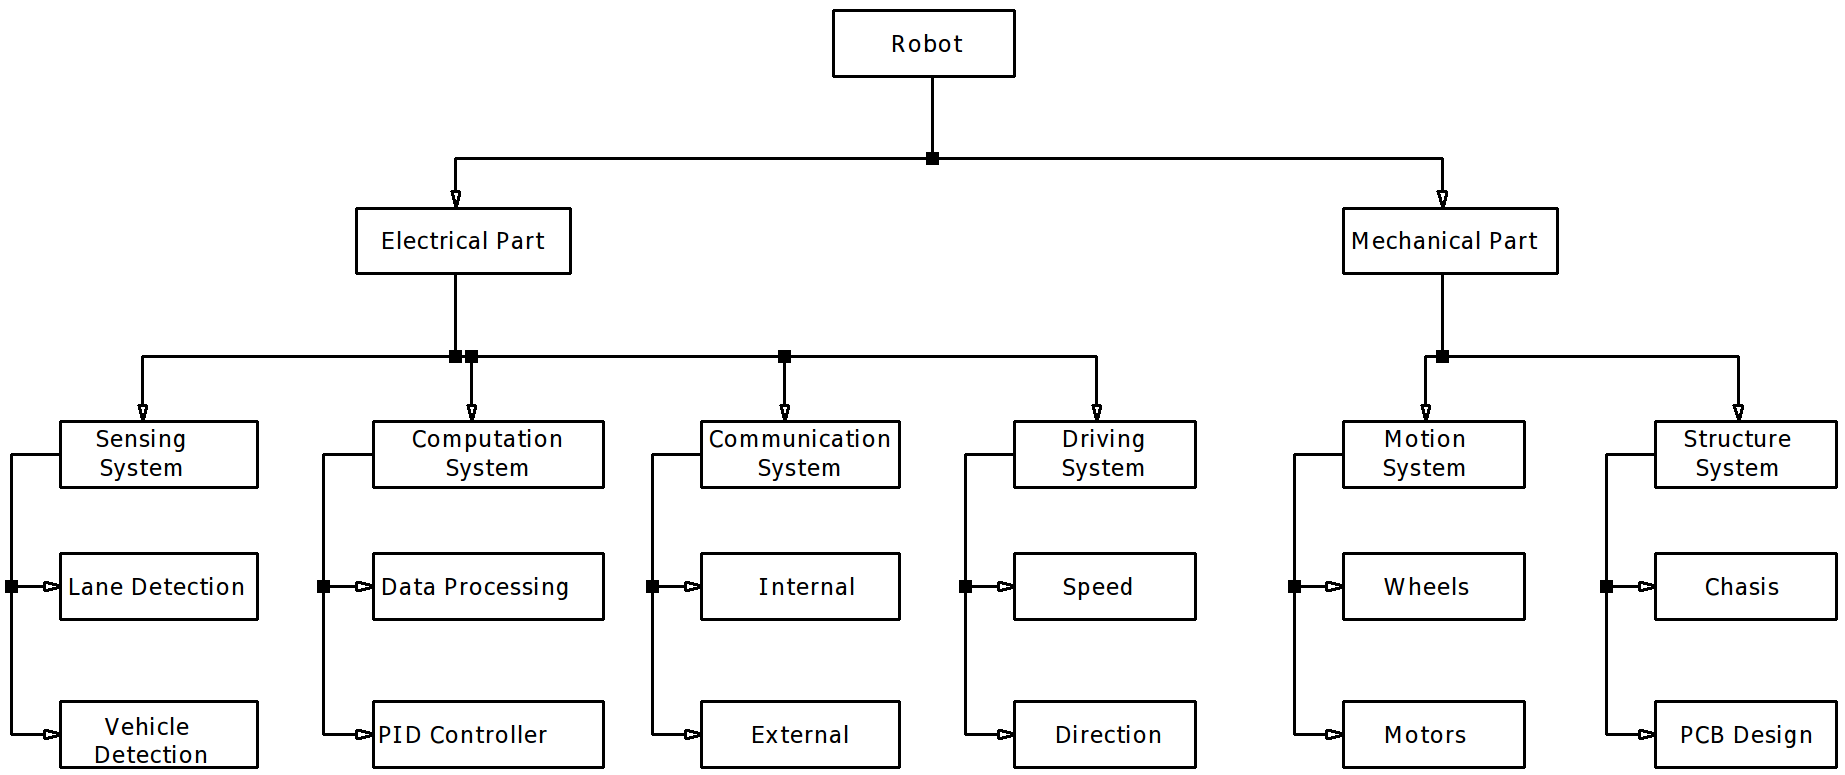
\includegraphics[width=\textwidth,center]{images/organization.png}
		\caption{System organization of the project}\label{fig:organization}
	\end{figure}
	
	\begin{enumerate}
		\item Sensing System
			
			This system is responsible for interpreting data from the environment. It has two subsystems namely,
			
			\subsection{Sensing System}
	
	Sensing system has two main subsystems which are Lane Detection subsystem and Vehicle Detection subsystem. The requirements of this subsystem are listed below:
	\begin{itemize}
		\item The system should detect the sides of the road.
		\item The system should not be effected from external disturbances.
		\item The system should detect the opponent vehicle.
	\end{itemize}
	
	
	\subsubsection{Lane Detection Subsystem}
	The subsystem basically detects the lane. This subsystem uses OpenCV libraries for processing camera frames. The input is captured from a Raspberry Pi camera that is mounted to the vehicle. The captured frame is firstly, preprocessed by a denoising filter and HSV color filter. The edges in the frame is detected by Canny Edge Detector algorithm. The output of Canny is a binary image filled with ones and zeros. The resulting binary image is processed with Hough Line detector to find pixels that possibly form a line. After the lines are found, the processed frame is sent to Data Processing subsystem. The block diagram of this subsystem is given in \textit{Figure~\ref{fig:lane_detection_subsystem}}. 
	
	
	\paragraph{Main Solution for Lane Detection Subsystem}
		
	The first processing on the captured frame is denoising by blurring. The blurring filter is a GaussianBlur of (3x3) matrix with zero variance both in x and y directions. Next, the filtered image is color filtered in HSV color space. The filter range of the HSV filter is adjusted only to include shades green. The lower bound for HSV filter is [H=60, S=120, V=106] and the higher bound is [H=82, S=255, V=235]. Later the color filtered image is processed by Canny Edge Detector. This process eliminates all pixels except those are constituting an edge. Edge pixels are usually formed when there is a transition from one object to other. To find pixels constituting a line, Hough Lines function is used.\\
	
	Hough Lines function outputs two pixels points on the image that form a line. The output of the function is tens of such line points. The accuracy of the function can be adjusted by playing with the input parameters. The function basically draws all lines that might go through a point in the free space (in polar coordinates) and intersects those lines. If the origin points of the intersected lines are within a specified bound, then the line is defined and it can be expanded further. If found points on a line don't exceed a threshold, that line is discarded. The adjustment of such parameters are done with trial and error approach. An important note is that this function is probabilistic, meaning that even if the input frame is never changed, the output line points would be close to previous point but not the same. An example call for this function together with its parameters is given \textit{Script~\ref{sc:hough-call}}. The output, line detected frame, is sent to Data Processing subsystem.
		\begin{lstlisting}[language=C++,float=h,numbers=left,frame=single,caption=Hough Lines Function with its Parameters, captionpos=b, label=sc:hough-call]
HoughLinesP(input=img_threshed, output=line,
rho=1, theta=CV_PI / 180, threshold=15, 
minLineLength=30, maxLineGap=40);
	\end{lstlisting}
	
	
	\subsubsection{Vehicle Detection Subsystem}
	
	The subsystem is the first step of safely competing with an opponent in a racing path. By the help of two distance sensors at the back and front of the vehicle the subsystem aims to find whether there is a opponent vehicle nearby.
	
	
	\paragraph{Main Solution for  Vehicle Detection Subsystem}
	
	 This subsystem uses two time of flight distance sensor which is enhanced IR sensor. One at the back of the vehicle responsible for detecting the chasing opponent and one at the front of the vehicle responsible for detecting the chased opponent. The subsystem produces positive output if the chasing vehicle or chased vehicle is within a range of 5 cm from the vehicle. Since the sensor reading is planned to be performed using Arduino, the required trigger for handshake protocol can be  easily send through serial commutation or directly implemented in the Arduino as an alternative. The requirements of this subsystem are listed below:
	
	\begin{itemize}
		\item The subsystem should detect the opponent to be caught with in a 5 cm 
		\item The subsystem should detect the chasing opponent if it reaches from back with in a 5 cm 
		\item The subsystem should trigger the handshake protocol 
	\end{itemize}
	
	
	
			
			\begin{enumerate}
				\item \textit{Lane Detection Subsystem} which is responsible for detecting sides of the path as its name suggests
				\item \textit{Vehicle Detection Subsystem} which is responsible for detecting opponent vehicle if it is close to the vehicle more than 5 cm
			\end{enumerate}
		
		\item Computation System
		
			This system is responsible for computational works of the vehicle. The system mainly give meaning to data generated by the sensing system. It has two subsystems namely,
			
			\begin{enumerate}
				\item \textit{Data Processing Subsystem} which is responsible for processing the output data of lane detection unit and produce data for PID control unit.
				\item \textit{PID Controller Subsystem} which is responsible for controlling the motors of the vehicle.
			\end{enumerate}
			
		\item Communication System	
		
		This system is responsible for communication inside the vehicle and communication between vehicles. It has two subsystems namely,
		
		\subsubsection{Data Processing Subsystem}
	
		The data processing subsystem is the main computation unit for the vehicle. The main objective of this subsystem is to give PID controller subsystem a meaningful data from unorganized data coming from lane detection subsystem. 
	
	\paragraph{Main Solution for Data Processing Subsystem}
	
	The input of this system is an edge detected binary image.  Next, points of the lines are classified as left or right borders of the lane. The elimination of the wrong points are done concurrently with the classification. Then, filtered points are fitted in two separate lines to create left and right borders of the lane. As the lane borders are found, the next and the last step is to determine the direction of the vehicle. The output of this subsystem is a turning angle and a direction. The whole process is summarized in \textit{Figure~\ref{fig:data_processing_subsystem}} as a block diagram. The requirements of this subsystem are listed below.\\
	
	Then next step is to classify the line points as left or right. The lines are firstly eliminated according to their slopes. If slope of a line is not in invalid slope region of $\pm$0.005, then it is a valid line. This process is done to get rid of unnecessary low sloped lines. After elimination, line points set must be determined as left or right. At this point, this classification is done according to double checking. The center of the image, that is 320th vertical pixel. If initial and final horizontal points of the image is in the same half, the line belongs to that half. This method works nicely in most regions of the path. However, it is a bit error prone in case of a sharp turning angle or losing one of the lanes . This algorithm will be improved to be more robust.
	\begin{lstlisting}[language=C++,float=t,numbers=left,frame=single,caption=The Algorithm to Classify the Lane Lines as Right or Left, captionpos=b, label=sc:left-right-lines]
std::vector<cv::Vec4i> lines // like a 4x4 matrix
double slope_thresh = 0.005; // absolute threshold slope
for (lines_points)
	startP = Point(x1, y1);
	endP = Point(x2, y2);
	line_slope = startP/endP;
	if(abs(line_slope) >= slope_thresh) line_is_valid;
	else line_is_not_valid;

for (lines_is_valid)	
	if(x1>320 && x2>320) it_is_right_line;
	else if(x1<320 && x2<320) it_is_left_line;
	else discard_the_line;
	\end{lstlisting}
	
	After finding the all left and right line points, actual left and right lines are constructed by applying the least square method to the both point sets. The result of this method is 4 points (x1,y1,x2,y2) to refer the left lane line and 4 points to refer the right lane line.
	
	The last process on the image is predicting the turn angle and direction. The prediction of direction is done by comparing the slopes of the left and the right lines. The turning is to be made to the side of the lane line having less slope. The angle is determined by computing the angle between the normal line of the current direction and guide line. Guide line is constructed with the average of the middle points of the right and the left lines and current point of the vehicle. Vehicle's current point is assumed to be in the middle of the beginning of the image. Thus, the beginning point of the guideline is the current position of the vehicle and the endpoint is the target point to be reached. The output of this processing is shown in \textit{Figure~\ref{fig:turn-prediction-explained}}. The turning angle and the direction is sent to PID Controller subsystem.
	
	
	\paragraph{Alternative Solutions for Data Processing Subsystem}
		The proposed algorithm for data processing has some flaws that are already discussed. To overcome those problems, DUAYENLER has some alternative solutions. An improvement might be on finding lane boundaries. This operation is currently realized with Hough Lines function. Another approach would be to scan rows an accurately edge detected image. If a white pixel is encountered, this would imply a lane boundary and the last time a white pixel is encountered would mean te other lane boundary. If the edge detected image contains noise, the solution might yield a wrong result. However, this can be overcomed by setting maximum number of white points that can be detected in a row.
		
		Another improvement could be on positioning on the lane. The proposed algorithm assumes that the vehicle follows the lane always in the center. This assumption is not the case always. The new algorithm will differentiate between the center of the lane and center of the capture image. By averaging coordinate points of both lane boundaries the actual lane center can be found and this point must be in some proximity with respect to the center of the image.
		
		\paragraph{Main Solution for PID Controller Subsystem}
	
		In our case the desired steady state error to be compensated by the controller is angle information coming from the data processing unit. For this purpose discrete time version of a general PID controller will be utilized. General form for discrete time PID controller may be seen below:
	
	$$ G_{PID}(z)=K_{bias}+K_p+K_I\frac{1}{1-z^{-1}}+K_D(1-z^-1)	$$
	
	Using bilateral Tustin transform where 
	
	$$ z=\frac{1+\overline{s}}{1-\overline{s}} $$
	
	The discrete time controller can be designed as if it is in continues domain.    
	
	
	
	
	
	
	\paragraph{Alternatve Solutions for PID Controller Subsystem}
		Theoretically very similar approach for designing a controller is to design in a S-domain. For this kind of controllers, general form of the continues time PID controller may be seen below:
		$$ G_{PID}(s)=K_{bias}+K_p+K_I\frac{1}{s}+K_Ds	$$
		
		Another alternative method is to design the controller directly in discrete domain without using bilateral Tustin transform. 
			
			\begin{enumerate}
				\item \textit{Internal Communication Subsystem} which is responsible for communication inside the vehicle mainly the communication between Raspberry Pi and Arduino.						\item \textit{External Communication Subsystem} which is responsible for the communication of the vehicle with the outside world mainly with the opponents.
			\end{enumerate}
		
		\item Driving System
		
		This system is responsible for the motion of the vehicle. Two parameters that are the direction and the speed of the vehicle is controlled by this unit accordingly to the information coming from controller. It has two subsystems namely,
			
			\begin{enumerate}
				\item \textit{Direction Subsystem} which is responsible for the orientation of the vehicle and keeps the road and the vehicle aligned.
				\item \textit{Speed Subsystem} which is responsible for the overall speed of the vehicle by adjusting it considering other effects on the vehicle.
			\end{enumerate}
			
		\subsubsection{Internal Communication Subsystem}
	This subsystem covers the communication of the components inside vehicle. Currently, Raspberry Pi and Arduino are two components that requires communication. To prevent the large amount of cable connection, a serial communication protocol is implemented. The requirements of this subsystem are listed below:
	\begin{itemize}
		\item The microcontrollers should be able to communicate with each other via serial communication
		\item The internal communication speed should be compatible with the processing speed of the lane detection subsystem  
	\end{itemize}
		\begin{lstlisting}[language=Python,float=h!,numbers=left,frame=single,caption=Serial object decleration in Python,label=sc:serial_python, captionpos=b ] 
import serial
ar=serial.Serial("/dev/ttyUSB0",9600)
		\end{lstlisting}
		 \begin{lstlisting}[language=C,float=h!,numbers=left,frame=single,caption=Serial communication setup in C,label=sc:serial_c, captionpos=b ] 
#include "./arduinoModule/rs232.h"
int cport_nr = 24; /* /dev/ttyUSB0 */
int bdrate = 9600; /* 9600 baud */
char mode[] = { '8', 'N', '1', 0 }; // 8 data bits, no parity, 1 stop bit
char str_send[2][BUF_SIZE]; // send data buffer
unsigned char str_recv[BUF_SIZE]; // recv data buffer
RS232_OpenComport(cport_nr, bdrate, mode);
		\end{lstlisting}
	\paragraph{Main Solution for Internal Communication Subsystem}
	
	There are several serial communication protocols that can be used to maintain the connection such as SPI, I2C. However, the first choice is to use USB serial port of the Arduino. Since RPi is practically a computer, it can recognize Arduino as a device using a serial port such as \lstinline|/ttyUSB0| in case of a Linux based OS. When recognized, RPi can send any piece of strings to the Arduino via USB cable. The process of communication is as follows:
	\begin{enumerate}
		\item Arduino should be connected to the Pi. \vspace{-0.2cm}
		\item Using Arduino IDE or any other method such as listing serial ports and checking for Arduino and so on, the serial port name should be detected \vspace{-0.2cm}
		\item Baud rates of two sides should be the same. 9600 is generally enough but if needed, it can be incremented to satisfy fast communication \vspace{-0.2cm}
		\item On Arduino side, \texttt{Serial.begin(9600)} command should be executed and serial port should be read repeatedly to capture the incoming data \vspace{-0.2cm}
		\item On Pi side, using any language C++ or Python, messages to serial port can be send 
	\end{enumerate}
	
	There are minor differences when implementing the code in Python, C++  and C. Python is the most practical one:\\
	
	Python has a library called serial by which any type of data can be send through serial ports. Script \ref{sc:serial_python} is used to declare a serial object. Then using \texttt{ar.write("some string \textbackslash r".encode())}, the string "some string" can be send to Arduino. Note that "\textbackslash r" carriage return character carries a high importance because it shows that a string is terminated and any other incoming data belongs to the new piece of string.   \\
	

	
	As alternatives, the implementation on C is also examined.	Sample codes to implement the same communication in C is in Script \ref{sc:serial_c}. Since it is a low level language, specification of buffer size and other parameters should be done in the code.\\

	%\lstinline[language=Arduino]|<SerialCommand.h>| 
	On Arduino  side, there are also several option that we can read the incoming data. Using \texttt{Serial.read()}  command is one of the simplest solutions. However, it contains some issues like conversion from string to integer and when to stop. Furthermore, the incoming data should be considered in character basis for the exact control.  
	
	\paragraph{Alternative Solutions for Internal Communication Subsystem}
		The communication between Raspberry Pi and Arduino can be realized by the use of other peripheral protocols or libraries.\\
	
		There is a \texttt{SerialCommand.h} library for the Arduino which allows executing a function depending on the incoming string. Using \lstinline|.addCommand("str",func)| of the library any function can be associated with any string coming from serial port. Moreover, the functions can have argument. For example, let the string "PWMSET" be execute a function \lstinline|setpwm()| but the PWM value is required. If incoming string is of the form "PWMSET 150", using \lstinline|.next()| function of the library, the value 150 can be read and converted into integer and interpreted as the PWM value to be set.\\
		
		Another solution is to use I2C or SPI protocols to set communication between Arduino and Raspberry Pi. These options require simple wiring connections between the pins. A point to remark is being cautious to operating voltage levels of pins of Arduino and Raspberry Pi.\\
		
		Besides aforementioned alternatives, Wi-Fi communication can also be considered between Arduino and Raspberry Pi. This solution requires deployment of a Wi-Fi module on Arduino. Some hardware exists in market such as ESP8266 and EMW3165. This solution would require a Wi-Fi network in the medium which makes the solution less implementable.\\
		
		A last solution would be to remove Arduino from the system. This would require the handover of operations of Arduino to Raspberry Pi. The resulting system could be considered as a single board solution, that is, all relevant subsystems operate on Raspberry Pi. This option would cause heating problems on Raspberry Pi. A cooling mechanism should also be applicable in this case.
		
		Communication subsystem enables the robot to communicate with the opponent using the handshake protocol agreed on standard committee. According to the standard committee, Wi-Fi modules must be used to implement handshaking. Since Raspberry Pi was used in the project, there is no need to get a separate Wi-Fi module; the internal Wi-Fi module of the Raspberry Pi was used.
	
	\paragraph{Main Solution for External Communication Subsystem}
	
	Socket programming is an effective tool to implement client-server communication algorithms. It can be implemented in Python or C++.  Our algorithms are written in Python for now, yet it can easily be converted to C++ if the team members decide that it is necessary. The algorithms for client and server sides are slightly different. \textit{Figure~\ref{fig:socket_funcs}} shows the functions that are used for client and server sides to create communication between client and server.
	
	
	
	Here is the summary of the key functions from socket library:
	
	\begin{itemize}
		\item socket.socket(): Creates a new socket using the given address family, socket type and protocol number.
		\item s.bind(address): Binds the socket to the address defined previously.
		\item s.listen(backlog): Sets up the maximum number of connections that can be made to the socket, which must be at 1 for the project.
		\item	s.accept(): Waits until connection arrives, then accept the client connection. Returns the client socket connected to the server as (conn, address) pair, where conn is a new socket object and address is the address bound to this socket
		\item	s.connect(): Provides client to connect to the server
		\item	s.send(): Transmits message to the remote socket.
		\item	s.recv(): Receives message from the remote socket
		\item	socket.close(): closes the socket; i.e., ends the communication with the opponent at the end of the race.
	\end{itemize}
	
	It is stated in the standard committee that each team must be assigned a static IP to communicate with the other robots. Duayenler has the static IP stated as “192.168.1.7” and the ID as “07”. Since Raspberry Pi 3 comes with a built-in wireless adapter, configuring it as a Wi-Fi hotspot is possible. To assign given IP to the robot, Raspberry Pi must be set as an access point from the terminal.\\
	
	In the algorithm that was implemented for the handshake, in a continuous loop, the front and rear sensors' values are been checked. There are two functions which are for client and server modes, respectively. If the front sensor senses the opponent in 5 cm range, our main code visits the client mode function. If the rear sensor senses the opponent in 5 cm range, server mode function runs. If our robot is in the server mode, the rear sensor value is again checked. The acknowledge message ($< ID> 01$) or reject message ($< ID> 11$) is sent according to the sensor value.
	
		\item Structure System
		
		This system is responsible for mechanical structure of the vehicle. Placement and orientations of both electrical and mechanical components are considered in this system. It has two subsystems namely,
		
		\paragraph{Main Solution for Direction Subsystem}
	Depending on the configuration of the wheels, exact control of the vehicle might vary. However, there are certain methods to accomplish orientation. The vehicle will definitely have two wheels or palettes that will be driven by two separate DC motors. That configuration allows differential drive method to orient the vehicle. PWM values of the motors can be adjusted such that the speed difference between them results in a turn as much as desired angle. The exact difference values on the PWM values depends on the specs of the used motors and voltage sources. 
	
	Two different H-bridge motor drivers are proposed to be used to drive DC motors: L298N and L293D. Both can drive two motors separately with one IC. However, maximum current rating of the former one is larger being 2A while L293D can supply 0.6A per channel. 
			
			\begin{enumerate}
				\item \textit{Chassis Subsystem} which is responsible for the connections of mechanical components in the vehicle.
				\item \textit{Printed Circuit Board Subsystem} which is responsible for the placement of electrical components.
			\end{enumerate}
			
		\paragraph{Main Solution for Speed Subsystem}
	Currently, there is no implementation for the subsystem because its operation depends on the control feedback loop and the success of the direction unit. Once they are operating and the vehicle is capable of following the lane at, least partially, then the speed subsystem will be implemented on top of the control algorithm.\\
	
	The best place to implement the state machine is Arduino as motor driving is also controlled by it. Main requirement for this system to operate is a measure of error or success for the direction subsystem. It can be the same as the error input of controller i.e. turning angle or a function of it. The state machine will act depending on the value of the error input. When it is above a critical level, the vehicle will show a steep deceleration to compensate the error of the direction unit. In other cases, It is wise to implement the speed controller in the form of at least PD controller. In other words, the change in the overall speed will also be maintained by a controller whose error input is not necessarily tried to be made zero but rather below a pre-specified level. State machine diagram can be seen in \textit{Figure \ref{fig:speed-state}}\\
		
		\item Motion System
		
		This system is responsible for maintaining mechanical feasibility of the driving system. It has two subsystems namely,
		
	\paragraph{Main Solution for Wheels Subsystem}
	
	The wheel placement combination that will be utilized is 2+1 combination. This combination can be assembled by placing 2 car wheels (with motors) to the back and the one boll caster to the front or vice versa. These configurations provide easy implementation and fairly reliable handling on the path. However, for certain obstacles may significantly disturb vehicles balance in this configuration.\\		
		
		\paragraph{Main Solution for Motors Subsystem}
	One of the widely used motor type is brushed gearhead DC motors. They are cheap and require enough torque for this competition. They have mainly two section one is the normal DC motor and gear head. Gear is a must to enhance torque performance of the DC motor. In other words, gear balance rpm and torque of the motor. 
			
			\begin{enumerate}
				\item \textit{Wheels Subsystem} which is responsible for the design of the wheel structure depending on the required speed-torque parameters.
				\item \textit{Motors Subsystem} which is responsible for the correct selection of the motor that is suitable to requirements.
			\end{enumerate}
	\end{enumerate}		
	
	General interaction of these subsystems with each other can be investigated at system diagram of the project at \textit{Figure~\ref{fig:system-diagram}}.
	
	
\paragraph{Main Solution for Chassis Subsystem}
	
	Current chasis structure relies on two pre-designed plexiglass layers. Raspberry Pi and Arduino is placed on the upper layer while motor driver and the battery are on lower one. To keep the center of mass of the vehicle close to the ground, battery is placed as low as possible. The connection of the motor driver and Arduino consists of eight cables two of which are the power lines. The cables are placed in a way that they cause no entanglement with any other parts. The connection between RPi and Arduino is currently accomplished by USB cable. \\
	
	Since there is not much component on the vehicle, the space on the layers are enough to locate the components. However, placing the camera of RPi has been a great problem. The view angle of the camera turned out to be considerable small than expected. Other several cellphone cameras were tried but they are could not satisfy the requirement that both side of the lane should be visible either. The only solution was to elevate the camera. That is why a camera holder structure is designed and added to the system.\\	
	
	To satisfy the requirements the holder is built using 4mm plexiglass. The choice satisfies the rigidity and light weight possible. A thinner one would result in less rigidity and increased vibration on the system. The designed structure, whose layout can be seen in \textit{Figure \ref{fig:camera-holder}}, has the elevation range from 35 cm to 45 cm and a camera angle ranging from $0^o$ to $45^o$. Having manufactured, the camera holder is integrated to the vehicle (\textit{see Figure \ref{fig:chassis}}). After integration, the view of the camera can completely cover the both edges of the path (\textit{see Figure \ref{fig:detection-test-results}})
	


	Current version of chassis which were used in critical module demo can be seen at \textit{Figure~\ref{fig:chassis}}.
	
	
	\subsubsection{Printed Circuit Board Subsystem}
	The main role of this part is decreasing connection mess and increase vibration strength of the robot against disturbances. Also, this section increases rigidity of the whole system. The requirements of this subsystem are listed below:	
	
This subsystem aims to make all the circuit connections rigid and compact. Currently, there is wire connections between Arduino-Motor driver and Arduino-RPi. However, addition of vehicle detection sensors and other lane detection alternatives will increase the amount of components, hence, wires. In addition, to use the space occupied by the Arduino UNO board, Arduino Mini can be used. This also allows to build the circuit board as shield for Arduino Mini. After that any other sensors and connections can be made through PCB. In other words, PCB acts as a breakout board for each item integrated to the system in a more rigid and compact way.
	
	
	
	\section{Detailed Requirements}
	
	
	
	\section{Detailed Solutions to Subsystems}
	
	V-Model is a very popular tool for system engineers to plan their projects. To ease the project tracking process, the V-Model was constructed by the DUAYENLER. The overall look of the V-Model can be seen at \textit{Figure~\ref{fig:vmodel}}. This section includes the explanation, requirements, test procedures and test results for the subsystems.
		
	


	The requirements of this subsystem are listed below:
	\begin{itemize}
		\item The subsystem should be able to detect only the shades of green color
		\item The subsystem should be able to detect edges in the camera frame in any light condition
		\item The subsystem should be able to tell differences between disturbances and lane
		\item The subsystem should be able to interpret the middle of the lane if both sides are present at the frame
	\end{itemize}
	
	
	
	\paragraph{Lane Detection Subsystem Tests}	
	The test procedure that will make sure correct functioning of this subsystem are list in the following sections.
	\begin{itemize}
		\item{Light Condition Test}
				\begin{enumerate}
				\item Mirror the Raspberry Pi screen into Laptop via VNC  \vspace{-0.2cm}
				\item Execute the lane detection algorithm in Raspberry Pi \vspace{-0.2cm}
				\item Change the location of the camera and Pi to conduct test \vspace{-0.2cm}
				\item Observe the results in different locations   \vspace{-0.2cm}
				\item If the visible lane sides can be detected without any additional object, the result of the test can be considered as success. \vspace{-0.2cm}
			\end{enumerate}
		\item{Visual Disturbance Test}
			\begin{enumerate}
			\item Mirror the Raspberry Pi screen into Laptop via VNC  \vspace{-0.2cm}
			\item Execute the lane detection algorithm in Raspberry Pi \vspace{-0.2cm}
			\item Put different objects into lane \vspace{-0.2cm}
			\item Observe the results with different disturbances\vspace{-0.2cm}
			\item If the objects outside of lane is not detected and the objects inside the road only detected only at its border with road, the result of the test can be considered as success. \vspace{-0.2cm}
		\end{enumerate}
	\end{itemize}
	
	\paragraph{Results of Lane Detection Subsystem Tests}
	
	The lane detection tests were conducted for the detection algorithm of the camera. The results were promising. The algorithm sweeps up the surrounding disturbances completely. The sample outputs together with Data Processing subsystem are shown in \textit{Figure~\ref{fig:detection-test-results}}.
	
	
	
		
			
	
	
		
	
	
	

	
	
	
	
		
	
	\paragraph{Vehicle Detection Subsystem Tests}\label{sect:vhd}
		
		\begin{itemize}
		
		\item Front Vehicle Detection Test in Closed Environment:
			This test aims to validate whether the subsystem is capable of detecting the opponent vehicle that is close to the vehicle more than 5 cm from the front. The test procedure is as follows; 		
			
			\begin{enumerate}
				\item Make the connection of the desired sensor and Arduino properly \vspace{-0.2cm}
				\item Hold the sensor at an angle of 90 degree with respect to ground \vspace{-0.2cm}
				\item Place the test object 5 cm in front of the desired \vspace{-0.2cm}
				\item Observe the output of the subsystem \vspace{-0.2cm}
				\item Repeat the step 3 \& 4 with different distances \vspace{-0.2cm}
				\item If the output of the subsystem generates logical positive for distances smaller than 5 cm and logical zero for distances greater than five, the test result can be considered as success \vspace{-0.2cm}
			\end{enumerate}					
		
		\item Rear Vehicle Detection Test in Closed Environment:
			This test aims to validate whether the subsystem is capable of detecting the opponent vehicle that is close to the vehicle more than 5 cm from the rear. The test procedure is as follows; 		
			\begin{enumerate}
				\item Repeat the test steps of the \textit{Front Vehicle Detection Test in Closed Environment} with the desired sensor for the desired rear sensor.  \vspace{-0.2cm}
			\end{enumerate}
		
		\item {Angled Approach Test:}
			This test aims to validate whether the subsystem is capable of detecting the opponent vehicle that is close to the vehicle more than 5 cm if the vehicles are not perfectly aligned. The test procedure is as follows;
			\begin{enumerate}
				\item Make the connection of the desired sensor and Arduino properly \vspace{-0.2cm}
				\item Hold the sensor at an angle of 90 degree with respect to ground \vspace{-0.2cm}
				\item Place the test object 5 cm in front of the sensor with 30 degree angle with respect to the sensor \vspace{-0.2cm}
				\item Observe the output of the subsystem \vspace{-0.2cm}
				\item Repeat the step 3 \& 4 with different distance and angle values \vspace{-0.2cm}
				\item If the output of the subsystem generates logical positive for distances smaller than 5 cm for all angle values with respect to sensor and logical zero for distances greater than 5 cm, the test result can be considered as success \vspace{-0.2cm}
			\end{enumerate}
		
		\item Vehicle Detection in Different Sunlight Conditions Test:
			This test aims to validate whether the subsystem is capable of detecting the opponent vehicle that is close to the vehicle more than 5 cm in different sunlight conditions. The test procedure is as follows; 		
			\begin{enumerate}
				\item Repeat the test steps of the \textit{Front Vehicle Detection Test in Closed Environment} in CCC (Cultural and Convention) ground under direct sunlight \vspace{-0.2cm}
				\item Repeat step 1 in CCC (Cultural and Convention) under artificial light, in other words, under no direct sunlight conditions \vspace{-0.2cm}
				\item Repeat steps 1 \& 2 for different locations of E Building including Graduation Laboratory \vspace{-0.2cm}
				\item If the output of the subsystem generates logical positive for distances smaller than 5 cm under all light conditions and logical zero for distances greater than 5 cm, the test result can be considered as success \vspace{-0.2cm}
			\end{enumerate}
			
		\end{itemize}
	
	\paragraph{Results of Vehicle Detection Subsystem Tests}
	
		All the test procedures mentioned at the \textbf{Section~\ref{sect:vhd}} were applied to the ultrasonic sensor (HC-SR04) and two infrared sensors (TCRT5000 \& QRD1114). The ultrasonic sensor were showed very inaccurate result especially in \textit{Angled Approach Test}. The test results can be examined at \textit{Table`\ref{tab:aat}}. Considering the fact that the path itself is elliptical and there would always be an angle between vehicle even though it may be very small for some cases, it was decided that ultrasonic sensors are not a good choice for this subsystem. However, it is always possible that these sensors can be supportive sensors for the subsystem.
		
		\begin{table}[H]
		  \centering
		  	\caption{The Results for the Angled Approach Test for HC-SR04}
		    \begin{tabular}{c|c|c}
    		   $$Actual Distance$$ & $$The Angle$$ & $$Measured Distance$$ \\ \hline
			   3  cm & 90 & 3.15 cm  \\ \hline
    		   5  cm & 90 & 5 cm  \\ \hline
    		   20 cm & 90 & 20.01 cm  \\ \hline
    		   40 cm & 90 & 40.25 cm \\ \hline
       		   5  cm & 45 & 6.78 cm \\ \hline
    		   20 cm & 45 & 28.8 cm  \\ \hline
       		   30 cm & 45 & 42.4 cm  
  			\end{tabular}
  			\label{tab:aat}
		\end{table}
		
		 Unlike ultrasonic sensors, infrared sensors showed very accurate result inside the closed environments like laboratory under artificial lights. However, the results under direct sunlight especially in CCC were not as good as expected.  Thus, it was decided that the main solution should be an enhanced version of infra-red sensors namely the ones utilizing the "time-of-flight" concept. Moreover, laser sensors might be good alternative for these subsystems.
		
	\subsection{Computation System}
	
	Computation system has two main subsystems which are Data Processing subsystem and PID Controller subsystem. The requirements of this system are listed below:
	\begin{itemize}
		\item The system should	be able to produce middle line to follow
		\item The system should be able to control the robot
	\end{itemize}	
	
		
	
	
	\textbf{Data Processing Subsystem Requirements:}	
	
	\begin{itemize}
		\item The subsystem should be able to analyze data produced by sensing system
		\item The subsystem should be able to produce the angle information required by the controller subsystem
		\item The subsystem should be able to work on Raspberry Pi
		\item The subsystem should be able to process one frame at most in 100 milliseconds
	\end{itemize}

	
		
	\paragraph{Data Processing Subsystem Tests}	
		This test will enable if data processing will generate the desired output, namely turn direction and angle. Test procedure is as follows:
		\begin{enumerate}
			\item Link the output of Lane Detection subsystem to Data Processing subsystem. \vspace{-0.2cm}
			\item Asses if the output coincide with physical reality of the path \vspace{-0.2cm}
		\end{enumerate}
	\paragraph{Results of Data Processing Subsystem Tests}
	The tests are done. The results are positive and reflects the expectations. The turn angle and direction are properly output. A flaw of this subsystem is that both right and the left lane lines must be determined. Otherwise, the prediction does not give stable results. This must be improved together with the Lane Detection subsystem regarding the code algorithm.	The sample outputs can be seen in \textit{Figure~\ref{fig:lane_detection_subsystem} and Figure~\ref{fig:turn-prediction-explained}}.
	
	\subsubsection{PID Controller Subsystem}
	
	The output of the data processing subsystem does not mean much for the rotating parts of the vehicle. The motors should be driven using some sort of closed loop system. PID controllers are the most used controller in the robotics field. The purpose of the PID controller is basically to eliminate the error from the desired steady state.The requirements of this subsystem are listed below:
	
	\begin{itemize}
		\item The subsystem should be able to control the motors
		\item The subsystem should be able to react the external disturbances
	\end{itemize} 
	
	
		
	\paragraph{PID Controller Subsystem Tests}	
	\begin{itemize}
		\item PID Parameters Test for Given Input:
			The test aims to speed up the process of finding the right PID parameters for the controller. The test procedure is as follows; 		
			\begin{enumerate}
				\item Connect the Vehicle Motors to Motor Controller \vspace{-0.2cm}
				\item Connect the Motor Driver to Arduino \vspace{-0.2cm}
				\item Give the angle value that the subsystem should compensate  \vspace{-0.2cm}
				\item Give the power to the motors \vspace{-0.2cm}
				\item Observe the behaviour of the vehicle \vspace{-0.2cm}
				\item If the vehicle rotates with an angle given in step 3 without any feedback given, the result of the test can be considered as success. \vspace{-0.2cm}
			\end{enumerate}
				
		
		\item Path Tracking Test:
			The test aims to check the validity of the PID parameters in closed loop feedback system. The test procedure is as follows; 		
			\begin{enumerate}
				\item Make the necessary connection between motors Arduino and data processing unit \vspace{-0.2cm}
				\item Place the vehicle to the desired empty path  \vspace{-0.2cm}
				\item Observe the behaviour of the vehicle \vspace{-0.2cm}
				\item If the vehicle can follow the path smoothly, the result of the test can be considered as success. \vspace{-0.2cm}
			\end{enumerate}
				
			
		\item Tracking a Path with Obstacles Test:
			The test aims to check the validity of the PID parameters in closed loop feedback system if there is obstacles. The test procedure is as follows; 		
			\begin{enumerate}
				\item Make the necessary connection between motors Arduino and data processing unit \vspace{-0.2cm}
				\item Place the vehicle to the desired path with obstacles \vspace{-0.2cm}
				\item Observe the behaviour of the vehicle \vspace{-0.2cm}
				\item If the vehicle can follow the path and compensate the steady state errors due to obstacles without showing oscillatory behaviour and in a reasonable time (in less than 2 seconds), the result of the test can be considered as success. \vspace{-0.2cm}
			\end{enumerate}
				
		
		\item Path Tracking Test with Physical Disturbances:
			The test aims to check the validity of the PID parameters in closed loop feedback system if there is a physical disturbance that effect the location of the vehicle. The test procedure is as follows; 		
			\begin{enumerate}
				\item Make the necessary connection between motors Arduino and data processing unit \vspace{-0.2cm}
				\item Place the vehicle to the desired empty path  \vspace{-0.2cm}
				\item Observe the behaviour of the vehicle \vspace{-0.2cm}
				\item If the vehicle can follow the path and compensate the steady state errors due to physical disturbance without showing oscillatory behaviour and in a reasonable time (in less than 2 seconds), the result of the test can be considered as success. \vspace{-0.2cm}
			\end{enumerate}
		
		\end{itemize}
	
		
		
	\paragraph{Results of PID Controller Subsystem Tests}
	
		Due to other limitations, the initial version of the PID controller subsystem was tested only for \textit{PID Parameters Test for Given Input}. The test results were promising for the time being. Other tests are planning to be conducted on the subsystem in the following semester.
	
	\subsection{Communication System}
	
	Communication system has two main subsystems which are Internal Communication subsystem and External Communication  subsystem. The requirements of this system are listed below::
	\begin{itemize}
		\item The subsystem should ensure safe internal communication
		\item The subsystem should ensure safe external communication
	\end{itemize}
	
	
	
	
	\paragraph{Internal Communication Subsystem Tests}
	This test will enable if communication between Arduino and Raspberry Pi can be realized. Test procedure is as follows:
	\begin{enumerate}
		\item Generate data on Raspberry Pi in a rate that reflects the time consumed of Data Processing subsystem. This will yield a realistic data rate. \vspace{-0.2cm}
		\item Send random text data to Arduino. \vspace{-0.2cm}
		\item Do the initial integration between Arduino and Raspberry Pi. \vspace{-0.2cm}
		\item Send data from Raspberry Pi to Arduino. \vspace{-0.2cm}
		\item Increase data speed to the specified data rate. \vspace{-0.2cm}
		\item Check the accuracy of the retrieved data.\vspace{-0.2cm}
	\end{enumerate}
	
	\paragraph{Results of Internal Communication Subsystem Tests}
	The results of the tests revealed that all steps are successful but the last step. The data send rate is determined to be 25 strings per second. The string length varies between one and three characters. The data is fully received if the rate is slower than 25 strings per second. However, the data loss  and  improper decoding is observed on the Arduino side. This must corrected by means of coding or switching to an alternative solution.
	
	\subsubsection{External Communication Subsystem}
	
	This subsystem covers basically the handshake protocol i.e. communication with the other vehicles on the path. The requirements of this subsystem are listed below:
	\begin{itemize}
		\item The subsystem should be able to communicate with the opponent via Wi-Fi protocol
		\item The subsystem should be able to execute handshake protocol
	\end{itemize}
	
	
	
	\paragraph{External Communication Subsystem Tests}
		
		\begin{itemize}
		
		\item Raspberry Pi as Client Test:
			This test aims to validate whether the Raspberry Pi can successfully fulfill the requirements set by \textit{Handshake protocol} as a client.Test procedure is as follows:
			\begin{enumerate}
				\item Create a hotspot from the computer \vspace{-0.2cm}
				\item Connect the Raspberry Pi to the hotspot \vspace{-0.2cm}
				\item Modify the client code to be tested according to IP address of the computer
				\item Run the server code from computer \vspace{-0.2cm}
				\item Run the client code from the Raspberry Pi \vspace{-0.2cm}
				\item Try the possible combinations from the terminals of both sides \vspace{-0.2cm}
				\item The test result can be considered as success if both sides respond according to the \textit{Handshake Protocol}.
			\end{enumerate}		
		
		\item Raspberry Pi as Server Test:
			This test aims to validate whether the Raspberry Pi can successfully fulfill the requirements set by \textit{Handshake protocol} as a client.Test procedure is as follows:
			\begin{enumerate}
				\item Create a hotspot from Raspberry Pi. \vspace{-0.2cm}
				\item Connect the computer to the hotspot \vspace{-0.2cm}
				\item Modify the client code to be tested according to IP address of the Raspberry Pi. \vspace{-0.2cm}
				\item Run the server code from Raspberry Pi. \vspace{-0.2cm}
				\item Run the client code from the computer. \vspace{-0.2cm}
				\item Try the possible combinations from the terminals of both sides \vspace{-0.2cm}
				\item The test result can be considered as success if both sides respond according to the \textit{Handshake Protocol}. 
			\end{enumerate}	
		
		\end{itemize}
		

	\paragraph{Results of External Communication Subsystem Tests}
	
	 The first and simplest test has been done on one computer (or raspberry pi) using the same device as client and server, at the same time. To achieve that, the computer's (or raspberry pi’s) IP address should be defined in the host section defined in the client mode function. Secondly, the codes were tested on two computers. Thirdly, one raspberry pi and one computer were used for the test. All tests were successful if the server side is connected to the internet and client side is connected to the server via hotspot. The outputs of the tests were given in the \textit{Figure~\ref{fig:handshake1}} and \textit{Figure~\ref{fig:handshake2}}.
	
	
	
	
	
	\subsection{Driving System}
	
	Driving system has two main subsystems which are Direction subsystem and Speed subsystem. The requirements of this system are listed below.\\
	
	\textbf{Driving System Requirements:}
	\begin{itemize}
		\item The subsystem should control motion subsystem according to output of the computation system
	\end{itemize}
	
	
	\subsubsection{Direction Subsystem}
	Direction unit is responsible for the orientation of the vehicle. It stores the last required orientation and the new one coming from the controller. After that, it tries to make the orientation as close as new one. Both data can be represented as vectors.The angle between those two vector is tried to be minimized by the controller. Before moving on to the operation, note that the angle can be used as a measure of the error that the direction unit have. The less the angle the more correctly operates the direction unit. The requirements of this subsystem are listed below:
	\begin{itemize}
		\item The subsystem should drive the motors according to computation system outputs
		\item The system should ensure that the vehicle follows the lane 
	\end{itemize}
	
	
	
	
	
	\paragraph{Direction Subsystem Tests}
	\begin{itemize}
	
		\item Straight Drive Test:
			This test aims to find the PWM bias between the two motors. The test procedure is as follows:
			\begin{enumerate}
				\item Make the necessary connections between motors, motor controller and the Arduino \vspace{-0.2cm}
				\item Set the PWM values of the motors equal \vspace{-0.2cm}
				\item Observe the behaviour of the motors \vspace{-0.2cm}
				\item Increase the PWM value of the slower motor until a point the vehicle can go in a straight line.
				\item Record this PWM difference to use in PID controller subsystem
			\end{enumerate}
				
			\newpage
		
		\item Circular Drive Test:
			\begin{enumerate}
				\item Make the necessary connections between motors, motor controller and the Arduino \vspace{-0.2cm}
				\item Desired curvature is decided \vspace{-0.2cm}
				\item  According to motion of the vehicle PWMs of the motors are set \vspace{-0.2cm}
				\item  PID parameters are set according to this test
			\end{enumerate}
		
		
	\end{itemize}
	
	\paragraph{Results of Direction Subsystem Tests}
		
		The test were conducted for the motor pairs used in the Critical Module Demo. The test can be repeated for new motor pairs if needed.
	
	
	\subsubsection{Speed Subsystem}
	
	This unit acts as a complementary module for direction unit. It will act as a state machine. In one state, the unit will try to increase the speed of the vehicle by making overall increase in both PWM values of DC motors. The feedback of this  system will be the cost function mentioned in driving unit. If that cost exceeds a specified level, unit goes to another state in which the unit will decrease the overall speed to allow direction unit to operate more correctly. In short, this unit tries to compensate the error of the direction unit by changing the overall speed of the vehicle. The requirements of this subsystem are listed below:
	\begin{itemize}
		\item The subsystem should decrease the vehicle speed at the narrow lane 
		\item The subsystem should increase the vehicle speed at the wide lane 
		\item The subsystem should decrease the vehicle speed at the extreme disturbance  
	\end{itemize}
	
	
	
	
	\paragraph{Speed Subsystem Tests}
	\begin{itemize}
		\item Determination of the error input: This test aims to find the correct error input for overall speed controllers. The test procedure is as follows:
		\begin{enumerate}
			\item Make all the necessary connection
			\item Start up the vehicle
			\item Execute lane detection and controller algorithms
			\item Set the error input of the both controller algorithms the same
			\item Observe the behavior
			\item Repeat the same process with a linear function of the input
			\item Observe the success of the tracking algorithm
		\end{enumerate}
		By checking in which case the vehicle is able to follow the path with less error, the error input can be decided.

		\item Determination of the critical error value: This test aims to specify above which error value, the emergency state should be triggered.
		\begin{enumerate}
			\item Make all the necessary connection
			\item Start up the vehicle
			\item Execute lane detection and controller algorithms
			\item While the vehicle is moving, give disturbance of different types
			\item Record the maximum value of the error encountered during the disturbances.
			\item Find the maximum value
		\end{enumerate}
		\end{itemize}
	\paragraph{Results of Speed Subsystem Tests}
	No test result is currently available due to mentioned reasons.

	\subsection{Motion System}
	
	Motion system has two main subsystems which are Wheels subsystem and Motors subsystem. The requirements of this system are listed below:
	\begin{itemize}
		\item The system should	ensure that the vehicle can drive itself with enough power
	\end{itemize}
	
	
	
	\subsubsection{Wheels Subsystem}
	There are possible solution for wheel placement on the chassis, and several wheel types. Some wheels are designed for better gripping on different surfaces. To avoids obstacles on the path, gripping of the wheel is an important concept. Some wheel types are ball caster, toy car wheel and palette. Besides, wheel placement and the wheel number should be combined with the wheel type choice. The requirements of this subsystem are listed below:
	\begin{itemize}
		\item The subsystem should ensure that the wheels can grip lane without slipping in all conditions 	
	\end{itemize}
	
	
	
	

	
	\subsubsection{Motor Subsystem}
	Motors are the one of the important physical components of the project. They represent the whole system's actions. As stated in the project definition, the path should be completed within 20 seconds and total length of the path is approximately 3 meters. Using this specifications, a simple calculation for RPM requirement yields
	\begin{equation}
	\begin{split}
	v=\frac{3}{20}&=\pi\times D\times\frac{RPM}{60}\\
	RPM&=\frac{2.865}{D}
	\end{split}
	\end{equation}
	where $D $ is the diameter of the wheels in meter. Currently used wheels has 6.5 cm diameter, which implies that RPM=44. This means that under load average RPM needs to exceed this value. To estimate torque value, it is necessary to predict components weight. When weight of the current components are measured, result is around 1kg, so rated torque of the each motor expected to 3 times larger than this value to obtain well acceleration in loaded condition. \\
	   
	The requirements of this subsystem are the followings:
	\begin{itemize}
		\item The subsystem should ensure that the motors can supply enough torque to accelerate the vehicle 
		\item The subsystem should ensure that the motors can execute driving system outputs without deviation
	\end{itemize}
	
	
	 
	
	 
	\paragraph{Motors Subsystem Tests}
	This unit’s test is focusing on two crucial parameters of the motor which are RPM and torque values of the motor. 
	Basic pulley system is used to calculate torque value of the motor.
	Distance is measured under the condition that at rated voltage and approximated load, to calculate loaded RPM value calculation.
	
	\paragraph{Results of Motors Subsystem Tests}
	The tests are done. The results are negative because motors torque value did not match with the declaration of the supplier. 3kg-cm is the decelerated value, but motors can only produce 750 g-cm. Therefore, this system is failed in torque requirement, and reconsidered in the following period. \\

		\begin{itemize}
			\item {Torque Test:} 
				\begin{enumerate}
					\item Fix the motor at horizontal position with respect to ground \vspace{-0.2cm}
					\item Attach an object of one kilogram \vspace{-0.2cm}
					\item Power up the motor \vspace{-0.2cm}
					\item Increase the weight to a point where the motor is not pulling anymore \vspace{-0.2cm}
					\item Record the value and check with expected results \vspace{-0.2cm}
					\item If the result is not comparable with expected values and very low, motor can be considered as broken \vspace{-0.2cm}
					\item Contact the seller for more information 
				\end{enumerate}
		\end{itemize}
	
	RPM test has not been done since torque value is not supporting test setup.
	\subsection{Structure System}
	
	Structure system has two main subsystems which are Chassis subsystem and Printed Circuit Board subsystem. The requirements of this system are listed below:
	\begin{itemize}
		\item The system should	ensure that structure is robust for external effects 
		\item The system should	ensure that structure is balanced
		\item The system should ensure that vehicle has a good appearance
	\end{itemize}
	
	
	
	\subsubsection{Chassis Subsystem}
	Main purposes of this subsystem are protection of the critical elements of the robot and holding components together. The most important part of this section is weight distribution. The chassis is supposed to be light and strong because of the competition purposes. However, it should balance the robot to be able to handle turns. The requirements of this subsystem are listed below:
	\begin{itemize}
		\item The subsystem should ensure that the chassis is rigid 
		\item The subsystem should ensure that the chassis have enough space for components
		\item The subsystem should ensure that the chassis can provide low center of mass 
	\end{itemize}
	
	
	
	The requirement for the camera holder can be listed as
	 \begin{itemize}
	 	\item It should be integrated to th front of the vehicle
	 	\item It should be as rigid as possible to reduce the vibration on the camera
	 	\item It should be light weight so that does not effect the center of mass considerably
	 	\item It should be adjustable in terms both elevation and camera angle
	 \end{itemize} 
	 
	 
	 
	
	
	\paragraph{Chassis Subsystem Tests}
	\begin{itemize}
		\item Inertia test: Aims to deduce a quantifiable measure of stabilization. Test procedure is as follows:
		\begin{enumerate}
		\item Prepare a straight path
		\item Power up the vehicle 
		\item Execute the edge detection and control algorithm
		\item Give different type of disturbances 
		\item Observe the deviation from straight line
		\item Repeat the process with different component configurations
		\end{enumerate} 
	\end{itemize}
	Currently no test results available due to lack of control algorithm.
	
	
	
	
	\begin{itemize}
		\item The subsystem should ensure that all the electronic components are placed on PCB
		\item The subsystem should ensure that all the connections are firmly secured and robust to vibrations.
	\end{itemize}
	
	





	
	\paragraph{Printed Circuit Board Subsystem Tests}
	Once completed, the board should be tested if it is built properly and correctly.
	\begin{itemize}
		\item Short test: Aims to check all the wanted connections are present. The test procedure is as follows:
		\begin{enumerate} 
			\item Open multimeter for short circuit test \vspace{-0.2cm}
			\item Find the ends of each routing 
			\item Check the continuity using multimeter probes
			\item Check if there is any unwanted short circuit
			\item If exist, eliminate
		\end{enumerate}
	\end{itemize}
	
	
	
	
	
	
	
	
	
	
	
	\section{Plans}
	Each team member is assigned to a subsystem according to their interest and qualification. \textit{Figure \ref{fig:plan-org}} summarizes the assignments. Besides, a Gannt Chart is prepared to have an detailed overview of future works and available in \textit{Appendix~\ref{gannt_chart_app}}.
	
	Future plans regarding the improvement of the project are listed here in system level.
	
	
	\subsection{Estimated Cost/Power of Project}
		Estimated cost anaysis for the project can be investigated at \textit{Table~\ref{tab:cost}}. The reproducible vehicle is expected to cost under 200 dollar as desired by the project requirements.
	
	\begin{table}[H]
  \centering
 	
 	\caption{Estimated Cost Analysis for the Project}
    \begin{tabular}{c|c}
       $$Component$$ & $$Price (in Dollar)$$  \\ \hline
       Raspberry Pi & 48   \\ \hline
       Camera & 23   \\ \hline
       Chassis & 20   \\ \hline
       Arduino & 5 \\ \hline
       Motors & 22 \\ \hline
       Wheels & 8 \\ \hline
       Motor Driver &  2.5 \\ \hline
       Powerbank & 12 \\ \hline
       Li-po Battery  & 15 \\ \hline
       Distance Sensors & 18 \\ \hline
       Additional Components & 10 \\ \hline
       Additional Payments & 15 \\ \hline
       Total Project &  198.5 
         
  
  \end{tabular} 
  \label{tab:cost}
  
\end{table}
		
		\newpage
	
	\section{Conclusion}
	
	\newpage
		\section{Disclaimer}
		\vspace{1cm}
		
		\textsf{ All information and content contained in this report are provided solely for proof-of-concept. DUAYENLER Ltd. Şti. guarantees that the report and information contained obeys the restrictions and rules ordered by the Standard Commitee.}
		
		\vspace{1cm}
		
		
		\begin{minipage}[b]{0.33\linewidth}
			\centering
			\underline{Halil TEMURTAŞ}
		\end{minipage}%
		\begin{minipage}[b]{0.33\linewidth}
			\centering
			\underline{Erdem TUNA}
		\end{minipage}%
		\begin{minipage}[b]{0.33\linewidth}
			\centering
			\underline{Enes TAŞTAN}
		\end{minipage} \\[2.5cm]
		
		\begin{minipage}[b]{0.495\linewidth}
			\centering
			\underline{Sarper SERTEL}
		\end{minipage}%
		\begin{minipage}[b]{0.495\linewidth}
			\centering
			\underline{İlker SAĞLIK}
		\end{minipage}\\[2.5cm]
		
		\begin{minipage}[b]{0.745\linewidth}
			\centering
			~~
		\end{minipage}%
		\begin{minipage}[b]{0.25\linewidth}
			\centering
			\underline{27 December 2018}
		\end{minipage}

\newpage

\begin{appendices}
	
%		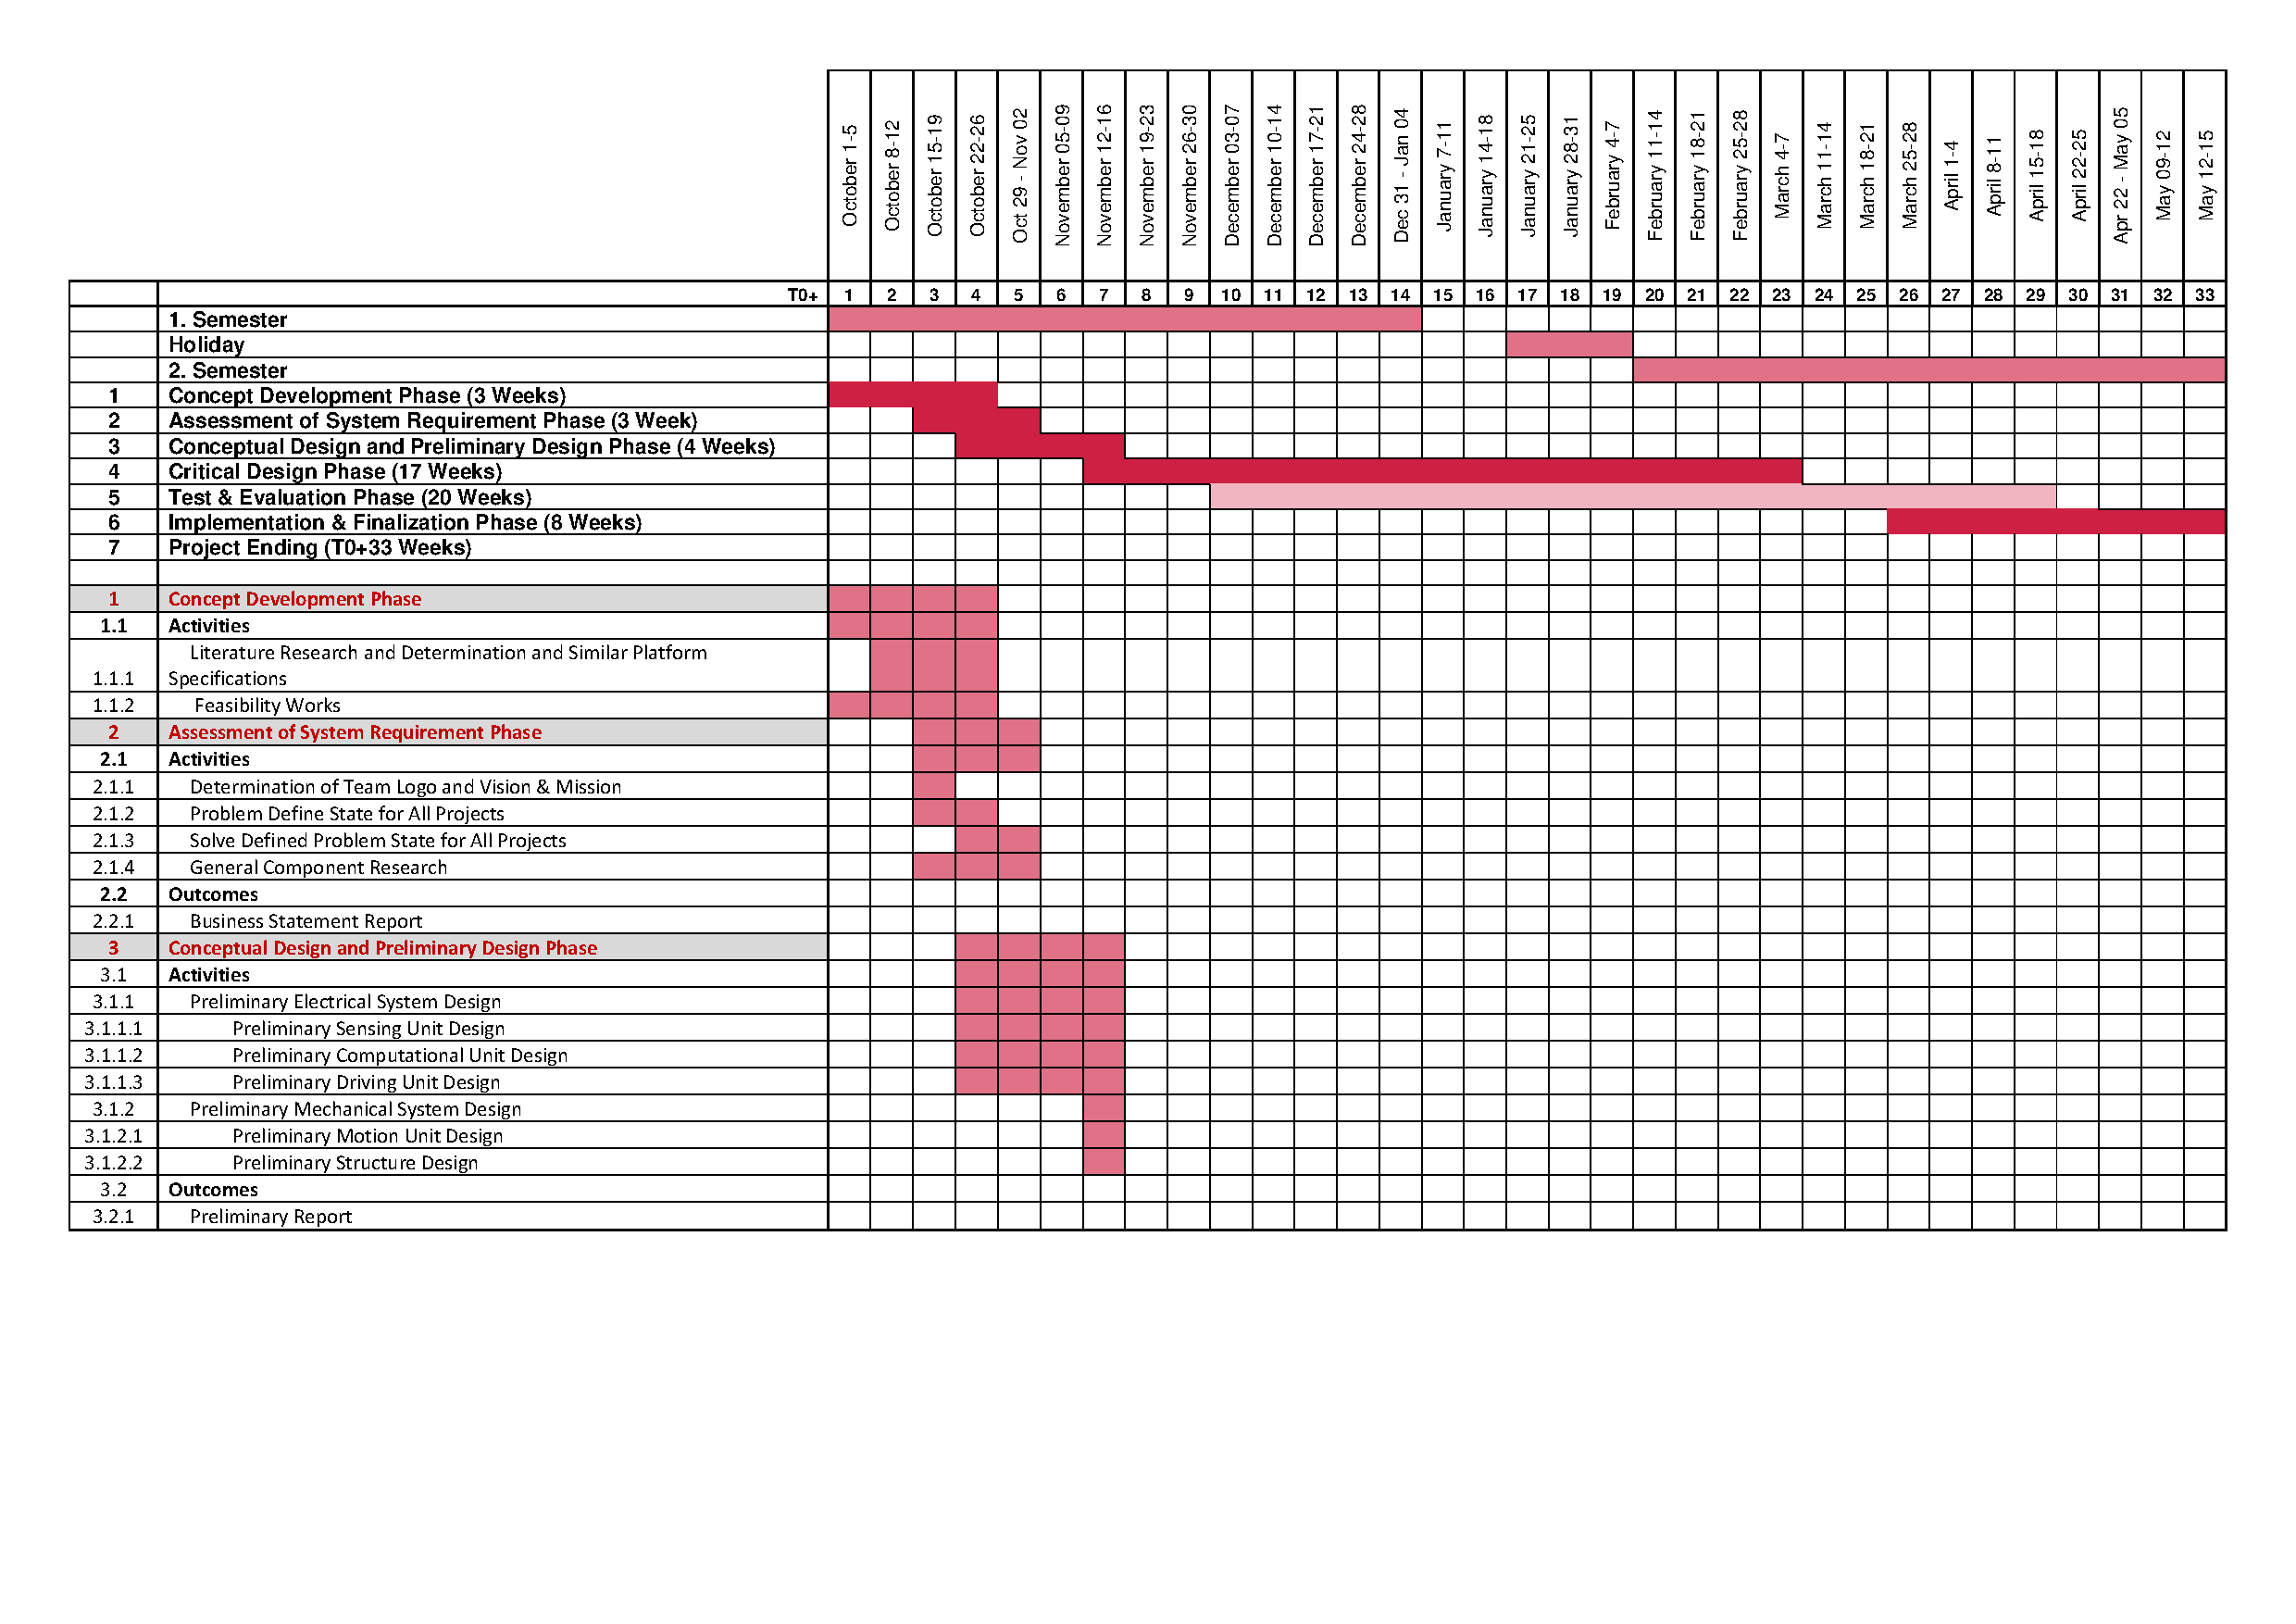
\includepdf[landscape=true,pages=1, scale=0.775,angle=0, label=gannt_chart_app,pagecommand=\section{Gannt Chart}\label{gannt_chart_app}]{gannt_chart.pdf}
%		\includepdf[landscape=true,pages=2-3, scale=0.775,angle=0,pagecommand=]{gannt_chart.pdf}

	
\end{appendices}




	
	
	
\end{document}

%----samples------
%\begin{itemize}
%\item Item
%\item Item
%\end{itemize}

%\begin{figure}[H]
%\center
%\setlength{\unitlength}{\textwidth} 
%
\includegraphics[width=0.7\unitlength]{images/logo1}
%\caption{\label{fig:logo}Logo }
%\end{figure}

%\begin{figure}[H]
%	\setlength{\unitlength}{\textwidth} 
%	\centering
%	\begin{subfigure}{.5\textwidth}
%  		\centering
%  		
\includegraphics[width=0.48\unitlength]{images/logo1}
%  		\caption{\label{fig:logo1}Logo1 }
%	\end{subfigure}%
%	\begin{subfigure}{.5\textwidth}
%  		\centering
%		
\includegraphics[width=0.48\unitlength]{images/logo2}
%  		\caption{\label{fig:logo2}Logo2}
%	\end{subfigure}
%\caption{\label{fig:calisandegree} Small Logos   }
%\end{figure}

%\begin{table}[H]
%  \centering
% 
%    \begin{tabular}{c|c|c}
%       $$A$$ & $$B$$ & $$C$$ \\ \hline
%       1 & 2 & 3  \\ \hline
%       2 & 3 & 4  \\ \hline
%       3 & 4 & 5  \\ \hline
%       4 & 5 & 6  
%      
%  \end{tabular}
%  \caption{table}
%  \label{tab:table}
%\end{table}

%\begin{table}[H]
%  \centering
% 
%    \begin{tabular}{c|c|c}
%       \backslashbox{$A$}{$a$} & $$\specialcell{ Average deviation \\ after subtracting out the  \\ frequency error }$$ & $$C$$ \\ \hline
%       \multirow{2}{*}{1} & 2 & 3  \\ \cline{2-3}
%        & 3 & 4  \\ \hline
%       3 & \multicolumn{2}{c}{4}  \\ \hline
%       4 & 5 & 6  
%      
%  \end{tabular}
%  \caption{table}
%  \label{tab:table}
%\end{table}
%-----end of samples-----
